% Options for packages loaded elsewhere
% Options for packages loaded elsewhere
\PassOptionsToPackage{unicode}{hyperref}
\PassOptionsToPackage{hyphens}{url}
\PassOptionsToPackage{dvipsnames,svgnames,x11names}{xcolor}
%
\documentclass[
  letterpaper,
  DIV=11,
  numbers=noendperiod]{scrreprt}
\usepackage{xcolor}
\usepackage{amsmath,amssymb}
\setcounter{secnumdepth}{-\maxdimen} % remove section numbering
\usepackage{iftex}
\ifPDFTeX
  \usepackage[T1]{fontenc}
  \usepackage[utf8]{inputenc}
  \usepackage{textcomp} % provide euro and other symbols
\else % if luatex or xetex
  \usepackage{unicode-math} % this also loads fontspec
  \defaultfontfeatures{Scale=MatchLowercase}
  \defaultfontfeatures[\rmfamily]{Ligatures=TeX,Scale=1}
\fi
\usepackage{lmodern}
\ifPDFTeX\else
  % xetex/luatex font selection
\fi
% Use upquote if available, for straight quotes in verbatim environments
\IfFileExists{upquote.sty}{\usepackage{upquote}}{}
\IfFileExists{microtype.sty}{% use microtype if available
  \usepackage[]{microtype}
  \UseMicrotypeSet[protrusion]{basicmath} % disable protrusion for tt fonts
}{}
\makeatletter
\@ifundefined{KOMAClassName}{% if non-KOMA class
  \IfFileExists{parskip.sty}{%
    \usepackage{parskip}
  }{% else
    \setlength{\parindent}{0pt}
    \setlength{\parskip}{6pt plus 2pt minus 1pt}}
}{% if KOMA class
  \KOMAoptions{parskip=half}}
\makeatother
% Make \paragraph and \subparagraph free-standing
\makeatletter
\ifx\paragraph\undefined\else
  \let\oldparagraph\paragraph
  \renewcommand{\paragraph}{
    \@ifstar
      \xxxParagraphStar
      \xxxParagraphNoStar
  }
  \newcommand{\xxxParagraphStar}[1]{\oldparagraph*{#1}\mbox{}}
  \newcommand{\xxxParagraphNoStar}[1]{\oldparagraph{#1}\mbox{}}
\fi
\ifx\subparagraph\undefined\else
  \let\oldsubparagraph\subparagraph
  \renewcommand{\subparagraph}{
    \@ifstar
      \xxxSubParagraphStar
      \xxxSubParagraphNoStar
  }
  \newcommand{\xxxSubParagraphStar}[1]{\oldsubparagraph*{#1}\mbox{}}
  \newcommand{\xxxSubParagraphNoStar}[1]{\oldsubparagraph{#1}\mbox{}}
\fi
\makeatother


\usepackage{longtable,booktabs,array}
\usepackage{calc} % for calculating minipage widths
% Correct order of tables after \paragraph or \subparagraph
\usepackage{etoolbox}
\makeatletter
\patchcmd\longtable{\par}{\if@noskipsec\mbox{}\fi\par}{}{}
\makeatother
% Allow footnotes in longtable head/foot
\IfFileExists{footnotehyper.sty}{\usepackage{footnotehyper}}{\usepackage{footnote}}
\makesavenoteenv{longtable}
\usepackage{graphicx}
\makeatletter
\newsavebox\pandoc@box
\newcommand*\pandocbounded[1]{% scales image to fit in text height/width
  \sbox\pandoc@box{#1}%
  \Gscale@div\@tempa{\textheight}{\dimexpr\ht\pandoc@box+\dp\pandoc@box\relax}%
  \Gscale@div\@tempb{\linewidth}{\wd\pandoc@box}%
  \ifdim\@tempb\p@<\@tempa\p@\let\@tempa\@tempb\fi% select the smaller of both
  \ifdim\@tempa\p@<\p@\scalebox{\@tempa}{\usebox\pandoc@box}%
  \else\usebox{\pandoc@box}%
  \fi%
}
% Set default figure placement to htbp
\def\fps@figure{htbp}
\makeatother





\setlength{\emergencystretch}{3em} % prevent overfull lines

\providecommand{\tightlist}{%
  \setlength{\itemsep}{0pt}\setlength{\parskip}{0pt}}



 


\KOMAoption{captions}{tableheading}
\makeatletter
\@ifpackageloaded{bookmark}{}{\usepackage{bookmark}}
\makeatother
\makeatletter
\@ifpackageloaded{caption}{}{\usepackage{caption}}
\AtBeginDocument{%
\ifdefined\contentsname
  \renewcommand*\contentsname{Table of contents}
\else
  \newcommand\contentsname{Table of contents}
\fi
\ifdefined\listfigurename
  \renewcommand*\listfigurename{List of Figures}
\else
  \newcommand\listfigurename{List of Figures}
\fi
\ifdefined\listtablename
  \renewcommand*\listtablename{List of Tables}
\else
  \newcommand\listtablename{List of Tables}
\fi
\ifdefined\figurename
  \renewcommand*\figurename{Figure}
\else
  \newcommand\figurename{Figure}
\fi
\ifdefined\tablename
  \renewcommand*\tablename{Table}
\else
  \newcommand\tablename{Table}
\fi
}
\@ifpackageloaded{float}{}{\usepackage{float}}
\floatstyle{ruled}
\@ifundefined{c@chapter}{\newfloat{codelisting}{h}{lop}}{\newfloat{codelisting}{h}{lop}[chapter]}
\floatname{codelisting}{Listing}
\newcommand*\listoflistings{\listof{codelisting}{List of Listings}}
\makeatother
\makeatletter
\makeatother
\makeatletter
\@ifpackageloaded{caption}{}{\usepackage{caption}}
\@ifpackageloaded{subcaption}{}{\usepackage{subcaption}}
\makeatother
\usepackage{bookmark}
\IfFileExists{xurl.sty}{\usepackage{xurl}}{} % add URL line breaks if available
\urlstyle{same}
\hypersetup{
  pdftitle={Sirojul Firdaus},
  pdfauthor={18224095 Sirojul Firdaus},
  colorlinks=true,
  linkcolor={blue},
  filecolor={Maroon},
  citecolor={Blue},
  urlcolor={Blue},
  pdfcreator={LaTeX via pandoc}}


\title{Sirojul Firdaus}
\usepackage{etoolbox}
\makeatletter
\providecommand{\subtitle}[1]{% add subtitle to \maketitle
  \apptocmd{\@title}{\par {\large #1 \par}}{}{}
}
\makeatother
\subtitle{Portfolio Asesmen II-2100 KIPP}
\author{18224095 Sirojul Firdaus}
\date{2025-10-22}
\begin{document}
\maketitle


\bookmarksetup{startatroot}

\chapter{Salam Hangat}\label{salam-hangat}

\includegraphics[width=6.14583in,height=\textheight,keepaspectratio]{images/headerkipp.png}

\section{Halo, sesama makhluk work in
progress!}\label{halo-sesama-makhluk-work-in-progress}

Hidup ini lucu, ya --- kita sering ngerasa udah ngerti arah, tapi
ternyata masih muter di tempat yang sama. Tapi nggak apa-apa, namanya
juga belajar. Kadang perlu tersesat sedikit buat tahu jalan pulang.

Santai aja, ini bukan CV atau surat lamaran kerja kok. Ini cuma aku ---
versi nggak formal dari seorang Sirojul Firdaus. Duduk santai, tarik
napas, dan yuk kenalan sebelum hidup keburu sibuk lagi hehe.

Katanya, masa kecil menentukan masa depan. Kalau benar begitu,
seharusnya aku sekarang jadi ketua geng motor. 😅 Untung hidup itu bisa
di-update, kayak software versi lama yang akhirnya sadar pentingnya
``perbaikan bug''. Jadi, ini bukan kisah orang sempurna, tapi kisah
orang yang lagi proses --- dari versi troublemaker 1.0 menuju Sirojul
2.0 (beta).

Di antara tawa, gagal, dan kopi sachet, aku belajar satu hal penting:
kadang hidup nggak perlu selalu lurus, yang penting nggak berhenti
melangkah.

Nah, kalau kamu udah siap, izinkan aku bercerita --- tentang masa kecil
yang absurd, perjuangan yang panjang, dan versi diri yang terus ku-debug
setiap hari. Cerita ini mungkin sederhana, tapi siapa tahu, kamu bisa
nemuongan dirimu di dalamnya. 😉

\part{Tugas Tengah Semester (UTS)}

\chapter{UTS-1 All About Me}\label{uts-1-all-about-me}

\includegraphics[width=4.16667in,height=\textheight,keepaspectratio]{All_About_me/../images/AZRL.png}

\section{Sebuah Awal yang Tidak
Manis}\label{sebuah-awal-yang-tidak-manis}

Aku bukan anak baik di masa kecil. Kalimat itu mungkin terdengar keras,
tapi biar jujur aja --- begitulah adanya. Sebelum kelas empat SD, aku
tumbuh di lingkungan yang, kalau boleh dibilang, bukan tempat ideal
untuk menanam mimpi. Hari-hariku diisi kenakalan, keisengan, dan rasa
penasaran yang sering berujung masalah. Hampir semua kenakalan remaja
pernah kucoba, kecuali dua hal:😅

Lucunya, justru dari masa itu aku belajar banyak. Hidup di lingkungan
yang ``berisik'' membuatku terbiasa membaca keadaan, memahami orang, dan
tahu kapan harus berhenti. Aku dulu tidak tahu arah, tapi entah
bagaimana, ada satu orang yang membuka mataku --- omku.

\section{Sebuah Percikan yang Mengubah
Segalanya}\label{sebuah-percikan-yang-mengubah-segalanya}

Omku bukan orang kaya, bukan juga lulusan universitas ternama. Tapi satu
kalimat darinya mengubah seluruh hidupku:

``Pendidikan bisa mengubah kualitas hidupmu, Us.''

Kalimat sederhana itu terasa seperti tamparan lembut. Untuk pertama
kalinya, aku sadar bahwa hidup bukan soal mengikuti arus, tapi tentang
memilih arah. Sejak itu, aku mulai melihat belajar bukan sebagai
kewajiban, tapi kesempatan.

Aku lahir di keluarga yang tidak akrab dengan kata ``edukasi''. Tak ada
yang bicara soal IPK, kuliah, atau riset. Tapi dari keluarga itu, aku
belajar arti perjuangan --- bahwa hidup bisa keras, tapi kita bisa lebih
keras lagi. Aku tumbuh dari minus: finansial yang serba pas-pasan, akses
pendidikan yang terbatas, dan lingkungan sosial yang kadang mematikan
mimpi. Tapi mungkin justru dari ``minus'' itulah semangatku berakar.

\section{Dari Minus}\label{dari-minus}

Aku tidak pernah bermimpi masuk ITB karena dulu rasanya tidak realistis.
Tapi mimpi kadang datang tanpa izin, dan usaha yang keras ternyata punya
suara. Aku menapaki jalan yang panjang --- penuh kegagalan, gap year,
dan rasa ragu --- hingga akhirnya aku berdiri di kampus ini, di STEI-K
ITB, belajar tentang sistem, teknologi, dan masa depan.

Aku memilih STEI-K karena di sanalah aku bisa menjembatani dua hal yang
paling kusukai: manajemen dan teknologi. Aku tertarik dengan data dan
AI, juga product management, di mana aku bisa menggabungkan logika,
kreativitas, dan empati untuk menciptakan solusi nyata.

Setiap hari di ITB, aku belajar bukan hanya teori, tapi juga cara
berpikir, bekerja dalam tim, dan memahami orang lain --- skill yang jauh
lebih penting dalam dunia nyata. Di sinilah aku belajar bahwa komunikasi
bukan sekadar berbicara, tapi tentang mengerti.

\section{Dari Anak Pemalas Menjadi
Eksplorator}\label{dari-anak-pemalas-menjadi-eksplorator}

Kalau ada yang bilang orang nggak bisa berubah, aku mungkin buktinya.
Dulu aku benci olahraga. Lari 500 meter aja bisa jadi tragedi. Tapi
entah kenapa, belakangan aku malah jadi orang yang nggak bisa diam:
badminton, futsal, gym, berenang, bersepeda. Sering aku mikir sendiri,
``Ini aku atau reinkarnasi orang lain?'' 😂

Tapi mungkin begitulah caraku menikmati hidup --- mencoba hal-hal baru
meski hanya sebentar. Aku tidak punya satu hobi tetap, tapi aku punya
semangat untuk terus mencari hal yang membuatku hidup. Aku menyebutnya
``exploring phase of life'' --- fase di mana aku belajar bahwa rasa
penasaran adalah bahan bakar paling murni untuk tumbuh.

\section{Antara Ekstrover dan
Introver}\label{antara-ekstrover-dan-introver}

Kalau kamu bertemu denganku di kampus, mungkin kamu akan mengira aku
ekstrover. Aku bisa bicara dengan siapa pun --- anak kecil, satpam,
dosen, bahkan direktur perusahaan. Tapi di sisi lain, aku juga suka
menyendiri, menikmati diam, atau sekadar menulis ide-ide yang melintas
di kepala.

Aku ambivert --- perpaduan dua dunia yang tampak bertolak belakang. Tapi
justru itu yang membuatku bisa menyesuaikan diri di banyak situasi.
Kadang aku yang memulai percakapan, kadang aku yang memilih
mendengarkan. Dari situ aku belajar satu hal: komunikasi bukan tentang
banyaknya kata, tapi tentang kehadiran.

\section{Belajar untuk Tidak Merasa
``Paling''}\label{belajar-untuk-tidak-merasa-paling}

Waktu SD dan SMP, aku selalu punya posisi aman --- si anak pintar yang
jarang gagal. Tapi saat masuk SMA, bahkan lebih lagi ketika kuliah, aku
sadar: dunia ini luas, dan banyak orang yang lebih hebat dariku.

Awalnya itu menampar ego. Tapi seiring waktu, aku menemukan ketenangan
baru --- kesadaran bahwa kita tidak harus menjadi yang paling hebat
untuk berarti. Yang penting adalah terus belajar, berproses, dan
konsisten menjadi lebih baik dari kemarin.

``I'm not the smartest in the room, but I'll make sure I'm the most
persistent.''

Kalimat itu kini jadi prinsipku. Aku bukan orang yang cepat paham, tapi
aku nggak akan berhenti sebelum paham.

\section{Kesadaran yang
Menyelamatkan}\label{kesadaran-yang-menyelamatkan}

Hal yang paling kusyukuri dalam hidup bukan pencapaian, tapi kesadaran
untuk sadar. Kedengarannya filosofis, tapi bagiku ini nyata. Di tengah
lingkungan masa kecilku yang rusak, aku bersyukur bisa punya kesadaran
untuk berkata pada diri sendiri, ``Aku bisa memilih arah berbeda.''

Kesadaran itu seperti lampu kecil di ruangan gelap --- nggak langsung
menerangi segalanya, tapi cukup untuk menemukan jalan. Dan buatku, itu
lebih dari cukup.

\section{Sedikit Tentang Rambut dan Hal-hal
Receh}\label{sedikit-tentang-rambut-dan-hal-hal-receh}

Kalau semua cerita di atas terlalu berat, mari istirahat sejenak 😄 Aku
punya satu kebiasaan aneh: aku nggak suka rambut panjang. Padahal banyak
cowok di teknik yang bangga sama rambut gondrongnya. Tapi aku? Begitu
rambut mulai nutupin telinga, aku langsung cari gunting. Aku nggak tahu
kenapa, tapi mungkin karena aku nggak suka sesuatu yang ``mengganggu
fokus.'' Hidup aja udah cukup rumit, ngapain nambah drama di kepala,
kan? 😆

\section{Menikmati Cerita Ini}\label{menikmati-cerita-ini}

Kalau ditanya apa harapanku dari tugas ini --- jujur aja, aku kerjain
karena tugas wkwkwk. Tapi kalau boleh berharap sedikit, aku ingin siapa
pun yang membaca atau menontonnya menikmati perjalananku. Nggak harus
merasa kasihan, nggak harus terinspirasi --- cukup tersenyum dan sadar
bahwa setiap orang punya versi perjuangannya sendiri.

Aku mungkin belum tahu akan jadi apa nanti. Tapi satu hal yang kutahu,
aku akan baik-baik saja. Karena aku sudah belajar hal paling penting:
bahwa perubahan dimulai dari keberanian untuk melangkah, bukan dari
hasil yang sudah pasti.

Someday, I'll become exactly who I'm meant to be. Dan perjalanan itu ---
sudah dimulai sejak aku berani berubah.

✨ End of UTS-1 ``All About Me'' -- Sirojul Firdaus ✨

\chapter{UTS-2 My Songs for You}\label{uts-2-my-songs-for-you}

NIKI - Take A Chance With Me

\url{https://youtu.be/iygXgP2nOF4?si=X9AWsynRQbwA8Wl5}

Lirik sudah ada di video.

\section{Sebuah Lagu yang
Mengingatkan}\label{sebuah-lagu-yang-mengingatkan}

Ada lagu yang dulu sering muncul entah dari mana. Kadang lewat playlist
acak, kadang lewat Locket yang kami pakai untuk saling kirim foto.
Judulnya Take a Chance with Me --- lagu lembut yang, bagi sebagian
orang, mungkin hanya tentang cinta. Tapi bagiku, lagu itu terdengar
seperti perjalanan; tentang keberanian kecil untuk melangkah meski tak
tahu akan sampai di mana.

Baitnya yang berbicara tentang seseorang yang berusaha menyembunyikan
perasaannya, atau tentang dua orang yang sama-sama takut mengaku, bukan
hanya tentang hubungan romantis. Aku mendengarnya sebagai metafora dari
perjuangan bersama --- dua orang (atau lebih) yang saling percaya dalam
diam, saling mendorong dalam letih, dan saling memahami meski tanpa
banyak kata.

\section{Masa yang Penuh Ritme}\label{masa-yang-penuh-ritme}

Lagu itu sering muncul di masa aku gap year --- masa di mana setiap hari
seperti latihan kesabaran. Kami belajar dari pagi sampai malam; kadang
diisi tawa, kadang kelelahan. Ada momen kami kelelahan menghitung
peluang di atas kertas, tapi tetap percaya peluang hidup selalu bisa
diubah dengan usaha.

Yang satu lebih jago bahasa, yang lain lebih paham logika. Kami saling
isi, saling ajar. Kadang serius, kadang saling mengejek soal rumus.
Pernah juga satu waktu aku sedikit (beneran seikit) lebih keras
menjelaskan konsep matematika --- niatnya baik, nadanya saja yang salah.
Hasilnya? air mata turun sebelum jawaban benar ditemukan. Tapi justru
dari situ aku belajar: pemahaman tanpa empati itu seperti hitungan tanpa
makna.

Dan setiap kali lagu itu muncul lagi, aku seperti diingatkan betapa
berharganya masa itu --- masa di mana ketegangan, tawa, dan mimpi
bercampur jadi satu.

\section{Antara Peluang dan
Keberanian}\label{antara-peluang-dan-keberanian}

Kalimat paling kuingat dari lagu itu adalah bagian yang berbunyi
kira-kira, ``In the end, we only regret the chances we didn't take.''
Lirik sederhana, tapi saat itu rasanya menampar lembut.

Dalam perjuangan menuju impian --- entah STEI-K atau FK --- setiap
keputusan terasa seperti ``mengambil kesempatan''. Tidak selalu pasti,
tidak selalu logis, tapi penuh harapan. Dan mungkin, take a chance di
sini bukan sekadar ajakan untuk berani mencintai, melainkan juga berani
percaya.

Percaya pada proses, percaya pada tujuan, dan percaya pada mereka yang
berjalan di sisi kita walau hanya sementara.

\section{Sebuah Lagu, Sebuah Ingatan}\label{sebuah-lagu-sebuah-ingatan}

Sekarang, setiap kali lagu itu muncul lagi, aku tidak hanya mengingat
seseorang, tapi masa --- masa ketika perjuangan masih sederhana: hanya
antara rasa ingin berhasil dan rasa takut gagal. Lagu ini seperti
pengingat lembut bahwa hal-hal berharga sering lahir dari pertemuan yang
tak direncanakan.

Aku belajar bahwa ``take a chance'' tidak selalu berarti menantang
dunia, kadang cuma berarti percaya sekali lagi, walau hati masih
gemetar.

\section{Penutup}\label{penutup}

Lagu ini tidak pernah berhenti terdengar, meski aku tak lagi
mendengarkannya sesering dulu. Mungkin karena lagu bukan sekadar bunyi,
tapi ruang tempat kenangan beristirahat dengan damai.

Dan jika ada satu pesan yang tersisa dari semuanya, mungkin begini:

Kadang, kesempatan tidak datang dua kali --- tapi kenangan dari
keberanian pertama akan terus bergema, seperti nada terakhir yang tak
benar-benar berakhir.

✨ End of UTS-2: ``My Song for You'' -- Sirojul Firdaus ✨

\chapter{UTS-3 My Stories for You}\label{uts-3-my-stories-for-you}

\textbf{Rumah yang Tak Selalu di Peta}

\section{Pembuka}\label{pembuka}

Ada yang bilang, rindu itu hanya milik mereka yang tinggal terlalu lama
di satu tempat. Tapi bagiku, rindu juga milik mereka yang terlalu sering
berpindah.

Setiap kota meninggalkan sedikit serpihan diri kita---aroma hujan, suara
orang lewat, langit yang warnanya unik di sore hari. Kadang kita nggak
sadar kapan sebuah tempat berhenti menjadi sekadar lokasi dan mulai
berubah menjadi ``rumah.''

Perjalanan hidupku seperti membuka peta yang warnanya selalu berubah.
Dulu, aku pikir ``perubahan'' itu tentang mencari tempat yang lebih
baik. Tapi ternyata, semakin jauh melangkah, aku malah makin sering
menoleh ke belakang.

\section{Surabaya}\label{surabaya}

Kalau bumi urutan ketiga dari matahari, mungkin Surabaya itu urutan
pertama. Panasnya bisa bikin es batu kehilangan semangat hidup dalam
lima menit. Tapi anehnya, justru di panas itu, aku tumbuh.

Ada aroma khas setelah hujan di Surabaya---campuran debu, tanah, dan
sesuatu yang tidak bisa dijelaskan, mungkin kenangan. Kadang, suara
qiroah sebelum maghrib terdengar lembut dari musholla dekat rumah,
diiringi bunyi motor lewat, dan obrolan ibu-ibu yang sedang menunggu
waktu berbuka. Simpel, tapi entah kenapa terasa hidup.

Aku masih ingat bagaimana suasana buka puasa di musholla: nasi bungkus
dibagikan, anak kecil berlarian, bapak-bapak ngobrol sambil kipas-kipas.
Aku duduk di pojok, menikmati suasana yang sama setiap tahun. Saat itu
aku nggak tahu bahwa rutinitas sekecil itu kelak akan kurindukan.

Lalu datang waktunya berpisah. Hari itu, aku berdiri di depan rumah
sambil menatap jalan yang sudah kuhafal setiap lubangnya. Perasaanku
campur aduk: excited karena akan ke kota baru, tapi juga sedih karena
meninggalkan segalanya. Aku bilang dalam hati, ``Surabaya, aku bakal
balik kalau udah berhasil.'' Entah kenapa, kalimat itu terdengar seperti
janji, meski aku nggak tahu kepada siapa.

Perjalanan menuju perubahan selalu terdengar keren sebelum dimulai. Aku
sempat berpikir: ``Akhirnya aku bisa keluar dari panas ini, keluar dari
lingkungan yang bikin aku stagnan.'' Kupikir, di luar sana semuanya
lebih segar, lebih inspiratif, lebih\ldots{} aku. Tapi ternyata, panas
Surabaya bukan cuma soal cuaca. Itu tentang kehidupan---tentang
bagaimana aku terbiasa ditempa dalam keadaan tidak nyaman tapi tetap
bisa tertawa.

Malam-malam mencari makan di pinggir jalan, nasi goreng gerobak
langganan, dan suara radio jadul dari warung sebelah---semuanya terasa
remeh waktu itu. Sekarang, kalau aku lihat video Surabaya di media
sosial, rasanya seperti melihat potongan diriku sendiri di sana, berdiri
di bawah lampu jalan sambil ketawa kecil. Aneh, ya? Dulu aku ingin
sekali pergi, sekarang malah ingin masuk ke layar itu dan bilang,
``tunggu sebentar, aku kangen.''

Tapi hidup memang seperti itu. Kadang, hal yang paling ingin kita
tinggalkan justru yang paling ingin kita datangi kembali. Dan aku baru
sadar, mungkin bukan Surabaya yang berubah---aku yang berubah.

\section{Jatinangor}\label{jatinangor}

Kalau Surabaya itu tentang panas yang menampar kulit, maka Jatinangor
adalah tentang udara pagi yang sejuk tapi diam-diam menusuk hati.

Saat pertama kali aku tiba di sana, aku sempat merasa kecewa. ``Ngapain
sih ITB di Nagor, bukan di Bandung?'' pikirku waktu itu. Aku
membayangkan kuliah di kota besar dengan kafe estetik, lampu-lampu
jalan, dan suasana urban yang sibuk. Tapi yang kutemukan justru jalan
menanjak, sawah di kejauhan, dan suara jangkrik malam hari.

Namun, waktu punya cara lucu untuk mempermalukan ekspektasi kita.
Semakin lama aku tinggal di Jatinangor, semakin aku sadar: tempat ini
pelan-pelan mengajarkanku untuk diam dan memperhatikan.

Setiap pagi, dari teras asrama, aku bisa melihat gunung di kejauhan.
Kadang berkabut, kadang jelas. Ada sesuatu yang magis dari pemandangan
itu --- seperti pengingat halus bahwa hidup nggak perlu tergesa-gesa.
Sore harinya, matahari tenggelam di balik bukit, memantulkan warna
jingga yang lembut di jendela kamar. Biasanya aku bengong saja di sana,
sambil mikir betapa lucunya hidup: aku dulu ingin meninggalkan panas,
tapi sekarang malah mencari kehangatan.

Kamar asrama kecilku sering jadi basecamp teman-teman dari kamar lain.
Entah bagaimana, kamar sempit itu bisa menampung banyak obrolan: tentang
masa depan, tentang nilai kuliah, bahkan hal-hal absurd yang nggak
penting sama sekali. Di situ aku belajar bahwa ``rumah'' bisa
sesederhana ruang di mana kamu bisa jadi dirimu sendiri tanpa takut
dihakimi.

Suatu malam, teman sekamarku pernah berkata sambil nyeruput kopi sachet,

``Lucu ya, dulu kita semua ngebet banget keluar dari kota masing-masing,
tapi sekarang malah pengen balik.''

Aku cuma tertawa kecil, tapi dalam hati aku tahu dia benar. Jatinangor,
dengan segala keterbatasannya, telah berubah dari ``tempat sementara''
menjadi ``tempat yang kurindukan.''

Mungkin karena di sana, semuanya terasa nyata. Kami saling bantu waktu
susah, saling curhat waktu stres, dan saling menertawakan hidup yang
belum tentu lucu. Dan di antara semua kesibukan kuliah dan organisasi,
aku selalu punya waktu untuk sekadar duduk di teras asrama, menatap
langit, dan berkata dalam hati, ``aku nyaman di sini.''

Lucunya, justru saat aku mulai nyaman, waktu berkata: ``Saatnya
pindah.'' Seperti biasanya, aku belum siap, tapi hidup nggak nunggu
kesiapan siapa pun. Aku harus berkemas, meninggalkan Jatinangor, dan
melangkah ke kota yang dulu kuimpikan --- Bandung.

\section{Bandung}\label{bandung}

Kalau Surabaya itu panas dan Jatinangor itu hangat, maka Bandung\ldots{}
agak sulit dijelaskan. Cantik, iya. Adem, iya. Tapi di balik itu semua,
ada rasa kosong yang tak pernah kuduga.

Bandung adalah kota dengan langit yang indah dan lalu lintas yang
membuatmu berpikir dua kali untuk keluar rumah. Setiap pagi, aku
melewati jalan yang penuh pohon, udara yang lebih bersih, dan
bangunan-bangunan yang tampak lebih ``modern.'' Di atas kertas, hidupku
di Bandung seharusnya lebih nyaman. Tapi kenyataannya, aku mulai merasa
kehilangan sesuatu yang bahkan tidak tahu apa.

Kontrakan yang kutempati sekarang sebenarnya bagus. Kamar luas, lokasi
strategis, lingkungan aman. Tapi anehnya, di rumah itu aku sering merasa
sepi. Mungkin karena dulu, di asrama, suasana selalu ramai. Ada suara
langkah kaki di lorong, tawa di malam hari, dan musik dari kamar sebelah
yang entah kenapa tidak pernah mengganggu. Sekarang, yang terdengar
hanya suara kipas angin dan detik jam dinding.

Aku pernah berpikir, ``Harusnya di sini lebih enak, kan? Bukannya ini
yang aku mau?'' Tapi ternyata, rumah yang ideal belum tentu terasa
seperti rumah. Aku belajar bahwa suasana bukan tentang fasilitas, tapi
tentang energi orang-orang di sekitarnya.

Kadang aku duduk sendirian di ruang tengah, menatap gelas kopi yang
uapnya mulai hilang, lalu tanpa sadar berpikir, ``Dulu di Jatinangor,
kopi sachet yang sama rasanya lebih nikmat.'' Bukan karena mereknya
beda, tapi karena dulu diminum bareng cerita, bareng tawa, bareng hidup.

Lucunya, di tengah kota yang katanya penuh warna ini, aku justru belajar
tentang hening. Hening yang bukan kosong, tapi ruang untuk memahami diri
sendiri.

Ada rasa yang pelan-pelan tumbuh: semacam penerimaan. Bahwa setiap
tempat memang punya waktunya. Surabaya mengajarkanku untuk bertahan.
Jatinangor mengajarkanku untuk menghargai kebersamaan. Dan Bandung ---
dengan segala sepinya --- mengajarkanku untuk berdamai dengan diri
sendiri.

\section{Refleksi Akhir}\label{refleksi-akhir}

Kadang aku berpikir, mungkin hidup itu seperti perjalanan dari kota ke
kota --- bukan untuk menemukan tempat terbaik, tapi untuk menemukan
versi terbaik dari diri kita di setiap tempat.

Surabaya, dengan panas dan kekacauannya, mengajarkanku arti ``tumbuh.''
Jatinangor, dengan kesejukan dan kesederhanaannya, mengajarkanku arti
``berbagi.'' Dan Bandung, dengan kesepiannya yang tenang, mengajarkanku
arti ``mengenal diri.''

Tiga tempat itu berbeda dalam segalanya --- cuaca, suasana,
orang-orangnya --- tapi ketiganya punya satu benang merah yang sama:
mereka semua pernah kuanggap bukan rumah, sampai akhirnya aku
merindukannya.

Dan mungkin di situlah letak ironi hidup: kita sering nggak sadar bahwa
kita sedang bahagia, sampai momen itu jadi kenangan. We only start
calling something ``home'' when it's no longer ours.

Dulu aku mengira ``rumah'' itu harusnya nyaman, tenang, dan sempurna.
Tapi kini aku tahu, rumah tidak harus begitu. Rumah bisa sesederhana
tempat di mana kamu merasa diterima, atau bahkan tempat di mana kamu
belajar menerima dirimu sendiri. Rumah tidak selalu punya koordinat di
peta --- kadang ia bersembunyi di hati orang-orang yang datang dan pergi
dalam hidupmu.

Kalau dipikir-pikir, rasa rindu itu bukti bahwa aku pernah benar-benar
hidup di tempat itu. Karena kamu tidak mungkin merindukan sesuatu yang
tidak pernah menyentuhmu, kan? Maybe that's why we keep moving --- bukan
karena ingin pergi, tapi karena kita tahu setiap tempat akan
meninggalkan sedikit versi diri kita di sana.

Dan saat semua perjalanan berakhir, kita akan menyadari bahwa ``rumah''
bukan hanya tentang tempat untuk kembali, tapi juga tentang keberanian
untuk terus melangkah.

Aku sering menatap peta digital di ponsel, memperbesar lalu memperkecil,
berpindah dari Surabaya ke Jatinangor lalu ke Bandung. Lucunya, garis
jarak di peta itu tidak pernah bisa menggambarkan jarak yang sebenarnya
--- jarak perasaan. Kadang hanya beberapa sentimeter di layar, tapi
terasa sejauh bertahun-tahun pengalaman dan perubahan diri.

Setiap kali aku menelusuri jalan virtual itu, aku senyum kecil sambil
berpikir: ``Jarak ini mungkin panjang, tapi semuanya tetap dalam
diriku.''

Dan aku rasa, itu cukup. Because maybe, home isn't where we stay ---
it's where we grow, and where we dare to leave, knowing we'll always
find our way back.

\section{Penutup}\label{penutup-1}

Sekarang, kalau ada yang bertanya di mana rumahku, aku mungkin akan
menjawab begini:

Rumahku bukan hanya di satu kota. Rumahku adalah di setiap tempat yang
pernah membuatku ingin pulang.

Karena pada akhirnya, hidup bukan tentang mencari tempat yang paling
nyaman, tapi tentang belajar nyaman di tempat yang kita miliki ---
setidaknya, untuk sementara waktu.

Dan kalau suatu hari aku pergi lagi ke kota lain, aku tahu satu hal:
rasa rindu ini akan datang lagi, mengingatkanku bahwa setiap tempat,
sekecil apa pun, pernah menjadi rumah --- meski hanya sebentar.

✨ End of ``My Stories for You'' -- Rumah yang Tak Selalu di Peta ✨ by
Sirojul Firdaus

\chapter{UTS-4 My SHAPE}\label{uts-4-my-shape}

Signature Strengths: Perseverance, Curiosity, Humor, Love of Learning,
Gratitude, Creativity, Empathy, Social Intelligence, Leadership, and
Spirituality. (Disintesis dari pengalaman hidup, refleksi diri, dan pola
kekuatan yang muncul dalam karya dan interaksi sehari-hari.)

\section{Ringkasan 1 Halaman}\label{ringkasan-1-halaman}

Peran Inti: Pembelajar dan perancang sistem yang mengubah konsep menjadi
karya nyata --- membangun solusi digital dan ekosistem belajar yang
bermakna. Misi: Menyalakan semangat belajar dan menghadirkan teknologi
yang membawa kebermanfaatan sosial. Kekuatan Utama: Ketelitian, empati,
kreativitas, daya juang tinggi, dan kemampuan menghubungkan ide dari
berbagai bidang. Dampak yang Dituju: Membentuk generasi yang paham
nilai, logika, dan kasih --- lewat teknologi yang adil, pendidikan yang
manusiawi, dan komunitas yang saling mendukung.

\section{S --- Spiritual Gifts}\label{s-spiritual-gifts}

Karunia terbesar saya adalah keteguhan hati dan kemampuan melihat makna
di balik setiap kesulitan. Saya belajar bahwa spiritualitas bukan hanya
soal doa, tapi juga soal bagaimana kita bertahan, memaafkan, dan terus
berbuat baik di tengah kekurangan. Dalam belajar maupun berkarya, saya
ingin menyalurkan semangat itu: bahwa bahkan dari kondisi yang rapuh,
sesuatu yang bernilai bisa tumbuh.

\section{H --- Heart (Minat dan Nilai
Hidup)}\label{h-heart-minat-dan-nilai-hidup}

Saya selalu tertarik pada teknologi yang menyentuh kehidupan nyata ---
terutama pendidikan dan pemberdayaan ekonomi. Saya percaya, literasi
digital bukan sekadar kemampuan teknis, tapi cara untuk membuka harapan.
Hati saya ada pada proses ``membuat orang lain mengerti,'' entah melalui
pengajaran, desain sistem, atau membangun aplikasi sederhana yang bisa
membantu orang lain. Saya ingin teknologi terasa manusiawi --- bukan
sekadar rumus dan kode, tapi juga jembatan bagi empati.

\section{A --- Abilities (Kemampuan
Andal)}\label{a-abilities-kemampuan-andal}

Saya cukup bisa dalam analisis logika, manajemen ide, dan desain sistem.
Saya juga punya ketelitian dan kesabaran yang tinggi --- dua hal yang
menolong saya saat menghadapi error di layar maupun ``error'' dalam
hidup. Saya terbiasa bekerja mandiri maupun berkolaborasi, berpikir
dalam pola besar tapi juga detail. Selain itu, kemampuan komunikasi dan
menulis reflektif membantu saya menyampaikan ide rumit dengan cara yang
sederhana dan bermakna.

\section{P --- Personality (Gaya Kerja dan
Kolaborasi)}\label{p-personality-gaya-kerja-dan-kolaborasi}

Saya reflektif, suka berpikir dalam, tapi juga adaptif terhadap
perubahan. Dalam tim, saya cenderung menjadi penghubung --- orang yang
menenangkan suasana dan mengarahkan fokus ke solusi. Saya bekerja paling
baik ketika punya ruang untuk berpikir bebas, tapi tetap punya tujuan
jelas. Saya menghargai proses lebih dari hasil instan, karena saya
percaya kualitas tumbuh dari perjalanan, bukan dari kecepatan.

\section{E --- Experiences (Pengalaman
Pembentuk)}\label{e-experiences-pengalaman-pembentuk}

Saya dibentuk oleh perjuangan dari bawah --- tumbuh dalam keterbatasan,
berjuang masuk ITB setelah gagal, dan belajar hidup jauh dari rumah yang
menjadi guru kesabaran. Setiap langkah membawa pelajaran: dari warung
kecil yang mengajarkan arti bertahan, dari gap year yang menanamkan
disiplin, sampai pertemanan yang membuat saya mengerti makna kolaborasi.
Semua itu mengajarkan saya bahwa keberhasilan bukan garis lurus --- tapi
lintasan penuh belokan yang membentuk arah hidup.

\section{Piagam Diri (Self-Charter)}\label{piagam-diri-self-charter}

Misi Hidup: Menggunakan ilmu dan teknologi untuk menumbuhkan manusia ---
bukan hanya cerdas, tapi juga berempati. Nilai Inti: Kejujuran,
Ketekunan, Empati, Keadilan, dan Rasa Syukur. Peran Inti: Pembelajar
seumur hidup, perancang sistem bernilai, dan mentor bagi mereka yang
ingin tumbuh. Kompas Keputusan: Apakah ini membawa manfaat bagi orang
lain? Apakah ini sejalan dengan nilai? Apakah saya masih menjadi manusia
yang bersyukur? Janji Pelayanan: Hadir sepenuh hati, bekerja dengan
makna, dan menebar keberanian untuk terus belajar meski dunia terasa
berat.

\section{Narasi 90 Detik --- ``Code of
Purpose''}\label{narasi-90-detik-code-of-purpose}

Saya Sirojul Firdaus --- mahasiswa STEI-K ITB yang belajar melihat dunia
bukan hanya lewat logika, tapi juga lewat rasa. Saya tumbuh dari
lingkungan sederhana, dari warung kecil tempat saya belajar tentang
tanggung jawab, sampai gap year yang mengajarkan arti sabar dan
konsistensi.

Bagi saya, teknologi bukan sekadar barisan kode, tapi cara untuk
memahami manusia --- cara untuk menjembatani kesenjangan antara tahu dan
peduli. Saya percaya, setiap baris program yang ditulis dengan niat baik
bisa jadi bentuk doa yang berjalan dalam sistem.

Saya punya mimpi: membangun ekosistem pembelajaran digital yang bisa
menyalakan semangat anak-anak dari daerah kecil --- agar mereka tahu
bahwa mimpi besar tidak hanya milik orang yang lahir di tempat besar.

Karunia saya ada pada kemampuan berpikir sistemik, mencipta, dan
mendengar. Saya ingin terus belajar, membimbing, dan menciptakan karya
yang bermakna --- bukan untuk sekadar berhasil, tapi untuk berguna.

Sebab, pada akhirnya, yang membuat hidup berharga bukan seberapa tinggi
kita naik, tapi seberapa banyak cahaya yang bisa kita bagi di sepanjang
perjalanan.

✨ End of UTS-4 ``My SHAPE'' -- Sirojul Firdaus ✨

\chapter{UTS-5 My Personal Reviews}\label{uts-5-my-personal-reviews}

\section{🧩 UTS-1 --- All About Me}\label{uts-1-all-about-me-1}

\begin{longtable}[]{@{}
  >{\raggedright\arraybackslash}p{(\linewidth - 6\tabcolsep) * \real{0.1875}}
  >{\raggedright\arraybackslash}p{(\linewidth - 6\tabcolsep) * \real{0.3250}}
  >{\raggedright\arraybackslash}p{(\linewidth - 6\tabcolsep) * \real{0.2125}}
  >{\raggedright\arraybackslash}p{(\linewidth - 6\tabcolsep) * \real{0.2750}}@{}}
\toprule\noalign{}
\begin{minipage}[b]{\linewidth}\raggedright
\textbf{Kriteria}
\end{minipage} & \begin{minipage}[b]{\linewidth}\raggedright
\textbf{Deskripsi Penilaian}
\end{minipage} & \begin{minipage}[b]{\linewidth}\raggedright
\textbf{Skor (1--5)}
\end{minipage} & \begin{minipage}[b]{\linewidth}\raggedright
\textbf{Catatan / Bukti}
\end{minipage} \\
\midrule\noalign{}
\endhead
\bottomrule\noalign{}
\endlastfoot
\textbf{Orisinalitas} & Cerita menunjukkan keaslian dan gaya khas
pribadi. & \textbf{4.9} & Gaya narasi humoris dan jujur seperti
``seharusnya aku jadi ketua geng motor''. \\
\textbf{Keterlibatan Emosional} & Pembaca dapat ikut merasakan
perjalanan batin penulis. & \textbf{5.0} & Emosi campur antara
perjuangan, refleksi, dan humor terasa kuat. \\
\textbf{Humor \& Ringan} & Ada unsur ringan yang membuat pembaca nyaman
membaca. & \textbf{4.8} & Gaya santai dan penuh kehangatan; tidak terasa
seperti tugas kuliah. \\
\textbf{Refleksi \& Insight} & Cerita mengandung pembelajaran dan
kesadaran diri. & \textbf{4.9} & Ada refleksi diri tentang perubahan dan
makna hidup. \\
\end{longtable}

\textbf{Total Skor: 4.9 (A)}\\
📝 \emph{Tulisan ringan tapi reflektif; menunjukkan self-awareness dan
kedewasaan berpikir.}

\begin{center}\rule{0.5\linewidth}{0.5pt}\end{center}

\section{🎵 UTS-2 --- My Songs for You}\label{uts-2-my-songs-for-you-1}

\begin{longtable}[]{@{}
  >{\raggedright\arraybackslash}p{(\linewidth - 6\tabcolsep) * \real{0.1875}}
  >{\raggedright\arraybackslash}p{(\linewidth - 6\tabcolsep) * \real{0.3250}}
  >{\raggedright\arraybackslash}p{(\linewidth - 6\tabcolsep) * \real{0.2125}}
  >{\raggedright\arraybackslash}p{(\linewidth - 6\tabcolsep) * \real{0.2750}}@{}}
\toprule\noalign{}
\begin{minipage}[b]{\linewidth}\raggedright
\textbf{Kriteria}
\end{minipage} & \begin{minipage}[b]{\linewidth}\raggedright
\textbf{Deskripsi Penilaian}
\end{minipage} & \begin{minipage}[b]{\linewidth}\raggedright
\textbf{Skor (1--5)}
\end{minipage} & \begin{minipage}[b]{\linewidth}\raggedright
\textbf{Catatan / Bukti}
\end{minipage} \\
\midrule\noalign{}
\endhead
\bottomrule\noalign{}
\endlastfoot
\textbf{Orisinalitas \& Relevansi} & Lagu dipilih dengan makna personal,
bukan sekadar favorit. & \textbf{4.8} & Lagu \emph{Take a Chance with
Me} dihubungkan dengan perjalanan perjuangan, bukan cinta semata. \\
\textbf{Keterlibatan Emosional} & Cerita menunjukkan hubungan emosional
dengan lagu. & \textbf{5.0} & Lagu menjadi pengingat perjuangan masa gap
year dan semangat bersama. \\
\textbf{Kedalaman Refleksi} & Lagu ditafsirkan dengan konteks kehidupan
nyata. & \textbf{4.9} & Penulis mengaitkan pesan lagu dengan motivasi
dan filosofi hidup. \\
\textbf{Gaya \& Kejelasan} & Tulisan mengalir dan mudah dipahami. &
\textbf{4.9} & Bilingual ringan, alami, dan berimbang antara rasa dan
refleksi. \\
\end{longtable}

\textbf{Total Skor: 4.9 (A)}\\
📝 \emph{Interpretasi lagu matang dan reflektif --- bukan sekadar
curhat, tapi pemaknaan mendalam.}

\begin{center}\rule{0.5\linewidth}{0.5pt}\end{center}

\section{📖 UTS-3 --- My Stories for
You}\label{uts-3-my-stories-for-you-1}

\begin{longtable}[]{@{}
  >{\raggedright\arraybackslash}p{(\linewidth - 6\tabcolsep) * \real{0.1875}}
  >{\raggedright\arraybackslash}p{(\linewidth - 6\tabcolsep) * \real{0.3250}}
  >{\raggedright\arraybackslash}p{(\linewidth - 6\tabcolsep) * \real{0.2125}}
  >{\raggedright\arraybackslash}p{(\linewidth - 6\tabcolsep) * \real{0.2750}}@{}}
\toprule\noalign{}
\begin{minipage}[b]{\linewidth}\raggedright
\textbf{Kriteria}
\end{minipage} & \begin{minipage}[b]{\linewidth}\raggedright
\textbf{Deskripsi Penilaian}
\end{minipage} & \begin{minipage}[b]{\linewidth}\raggedright
\textbf{Skor (1--5)}
\end{minipage} & \begin{minipage}[b]{\linewidth}\raggedright
\textbf{Catatan / Bukti}
\end{minipage} \\
\midrule\noalign{}
\endhead
\bottomrule\noalign{}
\endlastfoot
\textbf{Orisinalitas} & Cerita unik dan personal, bukan generik. &
\textbf{5.0} & Kisah tiga kota (Surabaya--Jatinangor--Bandung) sangat
otentik dan berlapis makna. \\
\textbf{Struktur \& Alur} & Cerita tersusun logis dengan transisi halus.
& \textbf{4.9} & Transisi antar bagian lancar; pembaca dibawa dengan
ritme yang konsisten. \\
\textbf{Pengembangan Emosi \& Diri} & Ada dinamika perasaan dan
pertumbuhan batin. & \textbf{4.8} & Dari ``ingin pergi'' jadi ``belajar
menghargai rumah''; reflektif dan lembut. \\
\textbf{Refleksi \& Pesan Akhir} & Cerita menutup dengan pesan
universal. & \textbf{4.9} & ``Rumah bukan tempat, tapi perasaan'' ---
kalimat yang filosofis dan kuat. \\
\end{longtable}

\textbf{Total Skor: 4.9 (A)}\\
📝 \emph{Narasi paling hidup dan puitis; tiap bagian menyatu dengan
transisi yang menarik.}

\begin{center}\rule{0.5\linewidth}{0.5pt}\end{center}

\section{🧠 UTS-4 --- My SHAPE}\label{uts-4-my-shape-1}

\begin{longtable}[]{@{}
  >{\raggedright\arraybackslash}p{(\linewidth - 6\tabcolsep) * \real{0.1875}}
  >{\raggedright\arraybackslash}p{(\linewidth - 6\tabcolsep) * \real{0.3250}}
  >{\raggedright\arraybackslash}p{(\linewidth - 6\tabcolsep) * \real{0.2125}}
  >{\raggedright\arraybackslash}p{(\linewidth - 6\tabcolsep) * \real{0.2750}}@{}}
\toprule\noalign{}
\begin{minipage}[b]{\linewidth}\raggedright
\textbf{Kriteria}
\end{minipage} & \begin{minipage}[b]{\linewidth}\raggedright
\textbf{Deskripsi Penilaian}
\end{minipage} & \begin{minipage}[b]{\linewidth}\raggedright
\textbf{Skor (1--5)}
\end{minipage} & \begin{minipage}[b]{\linewidth}\raggedright
\textbf{Catatan / Bukti}
\end{minipage} \\
\midrule\noalign{}
\endhead
\bottomrule\noalign{}
\endlastfoot
\textbf{Kelengkapan SHAPE} & Semua bagian (S--H--A--P--E) terisi lengkap
dan jelas. & \textbf{5.0} & Setiap elemen disusun sinkron dan relevan
dengan perjalanan hidup. \\
\textbf{Koherensi \& Keterkaitan} & Nilai, kemampuan, dan pengalaman
saling terhubung. & \textbf{4.9} & Karunia spiritual, minat, dan
pengalaman dikaitkan secara logis. \\
\textbf{Keaslian \& Kejujuran} & Tulisan menunjukkan pemahaman diri yang
tulus. & \textbf{4.8} & Refleksi tidak dibuat-buat; menggambarkan
identitas sejati penulis. \\
\textbf{Gaya \& Inspirasi} & Bahasa jelas, reflektif, dan inspiratif. &
\textbf{4.9} & Ringkas, namun menggerakkan dan mudah dibaca. \\
\end{longtable}

\textbf{Total Skor: 4.9 (A)}\\
📝 \emph{Refleksi diri yang solid dan berisi; terasa tulus dan seimbang
antara logika dan hati.}

\begin{center}\rule{0.5\linewidth}{0.5pt}\end{center}

\section{\texorpdfstring{📊 \textbf{Rekap Nilai
Keseluruhan}}{📊 Rekap Nilai Keseluruhan}}\label{rekap-nilai-keseluruhan}

\begin{longtable}[]{@{}
  >{\raggedright\arraybackslash}p{(\linewidth - 8\tabcolsep) * \real{0.1111}}
  >{\raggedright\arraybackslash}p{(\linewidth - 8\tabcolsep) * \real{0.2222}}
  >{\raggedright\arraybackslash}p{(\linewidth - 8\tabcolsep) * \real{0.2556}}
  >{\raggedright\arraybackslash}p{(\linewidth - 8\tabcolsep) * \real{0.1889}}
  >{\raggedright\arraybackslash}p{(\linewidth - 8\tabcolsep) * \real{0.2222}}@{}}
\toprule\noalign{}
\begin{minipage}[b]{\linewidth}\raggedright
\textbf{UTS}
\end{minipage} & \begin{minipage}[b]{\linewidth}\raggedright
\textbf{Kriteria Utama}
\end{minipage} & \begin{minipage}[b]{\linewidth}\raggedright
\textbf{Skor Total (1--5)}
\end{minipage} & \begin{minipage}[b]{\linewidth}\raggedright
\textbf{Nilai Huruf}
\end{minipage} & \begin{minipage}[b]{\linewidth}\raggedright
\textbf{Deskripsi Umum}
\end{minipage} \\
\midrule\noalign{}
\endhead
\bottomrule\noalign{}
\endlastfoot
🧩 \textbf{UTS-1: All About Me} & Orisinalitas, Emosi, Humor, Insight &
\textbf{4.9} & \textbf{A} & Penuh karakter, jujur, dan reflektif. \\
🎵 \textbf{UTS-2: My Songs for You} & Orisinalitas, Emosi, Refleksi,
Gaya & \textbf{4.9} & \textbf{A} & Lagu dijadikan refleksi perjuangan
hidup. \\
📖 \textbf{UTS-3: My Stories for You} & Struktur, Emosi, Refleksi,
Orisinalitas & \textbf{4.9} & \textbf{A} & Cerita perjalanan diri yang
menyentuh dan jujur. \\
🧠 \textbf{UTS-4: My SHAPE} & SHAPE, Koherensi, Keaslian, Inspirasi &
\textbf{4.9} & \textbf{A} & Piagam diri yang matang dan autentik. \\
\end{longtable}

\textbf{💯 Nilai Akhir Keseluruhan: 19.6 / 20 --- (98\%) --- A (Sangat
Baik)}\\
\textgreater{} ``Tulisan yang tidak hanya menjawab tugas, tapi
menggambarkan perjalanan hidup dengan kedalaman dan kejujuran.''

\section{EXCEL PEER ASSIGNMENT}\label{excel-peer-assignment}

\href{https://docs.google.com/spreadsheets/d/1qMTxE2IL-6VU3V1p_5wxtJhy2ml_Fibt/edit?usp=sharing&ouid=111994471425383838960&rtpof=true&sd=true}{Klik
di sini untuk membuka Google Sheet}

\part{Tugas Akhir Semester (UAS)}

\chapter{UAS-1 My Concepts}\label{uas-1-my-concepts}

\textbf{Pulse of The Planet: Menyelaraskan Detak Jantung Global Lewat
TISE}

\begin{figure}[H]

{\centering 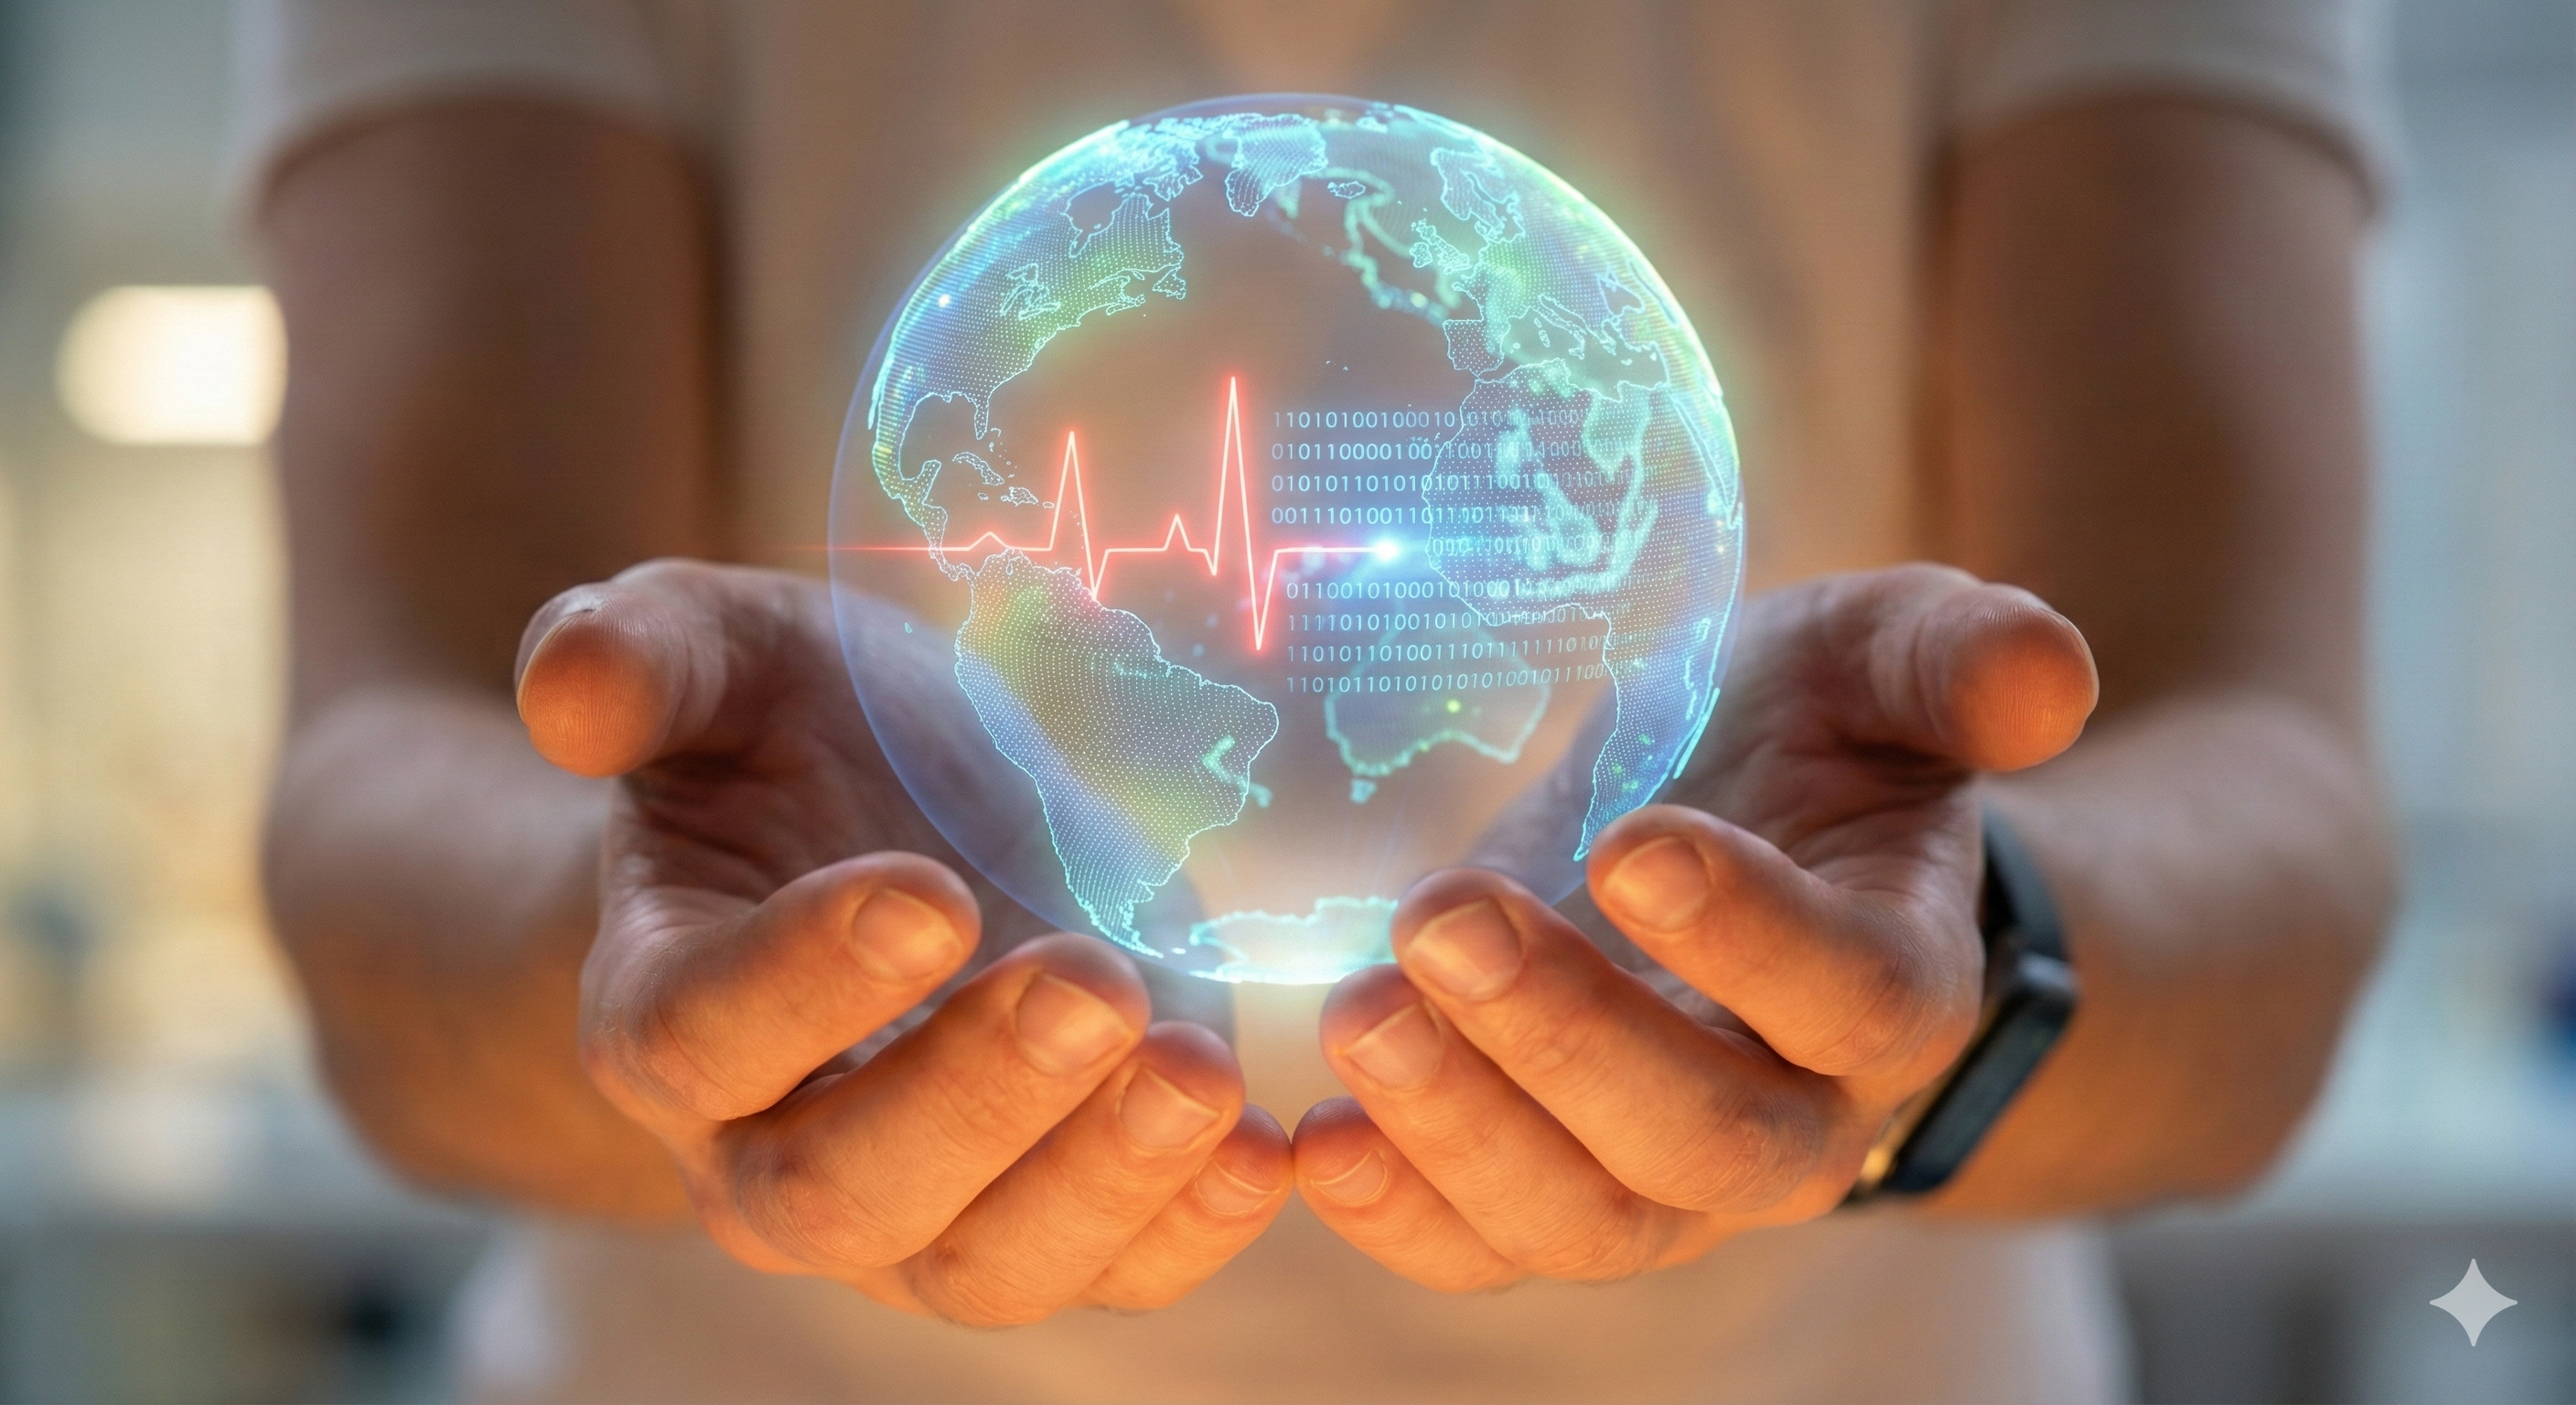
\includegraphics[width=1\linewidth,height=\textheight,keepaspectratio]{My_Concepts/../images/pulse_planet.png}

}

\caption{Pulse of The Planet}

\end{figure}%

\section{Refleksi dari ``Minus'': Ketika Sehat adalah
Kemewahan}\label{refleksi-dari-minus-ketika-sehat-adalah-kemewahan}

Tumbuh di lingkungan yang ``berangkat dari minus'' mengajarkan aku satu
hal pahit: kesehatan adalah benteng pertahanan terakhir sebuah keluarga.
Ketika sakit menyerang keluarga yang rentan, ia bukan hanya masalah
medis, tapi bencana ekonomi.

Aku melihat data ini bukan sekadar angka: 4,5 miliar manusia---separuh
populasi bumi---belum mendapatkan layanan kesehatan esensial, dan
ratusan juta jatuh miskin hanya karena berusaha untuk sembuh. Bagi
mereka, dan bagi masa laluku, sehat adalah sebuah \emph{privilese},
bukan hak.

Konsep ``Mahakarya'' yang aku tawarkan bukanlah tentang menciptakan
robot canggih yang menggantikan sentuhan manusia, melainkan sebuah
\textbf{Sistem TISE (Triune-Intelligence Smart Engineering)} yang
mendemokratisasi akses. Aku menamainya \textbf{``Pulse of The Planet''}
(Detak Jantung Planet)---sebuah upaya menyelaraskan tiga komponen
kecerdasan agar jantung kemanusiaan tetap berdetak, tak peduli seberapa
``minus'' kondisi ekonominya.

\section{Arsitektur TISE: Pulse of The
Planet}\label{arsitektur-tise-pulse-of-the-planet}

Untuk menggerakkan 8 miliar manusia menuju keadilan kesehatan, kita
perlu menyelaraskan tiga elemen fundamental:

\subsection{\texorpdfstring{1. Hati (Kecerdasan Manusia /
\emph{Homocordium}) --- \emph{The Compass of
Care}}{1. Hati (Kecerdasan Manusia / Homocordium) --- The Compass of Care}}\label{hati-kecerdasan-manusia-homocordium-the-compass-of-care}

Ini adalah \textbf{Axiological Intelligence (AQ)} kolektif kita. Dalam
konteks kesehatan global, ``Hati'' adalah kompas moral yang berteriak
bahwa akses kesehatan adalah hak asasi.

\begin{itemize}
\tightlist
\item
  \textbf{Masalah:} Kita mengalami krisis empati. Teknologi medis maju,
  tapi distribusinya macet karena motif profit.
\item
  \textbf{Konsep TISE:} \emph{Homocordium} berfungsi menentukan
  ``Mengapa'' kita bertindak. Tanpa Hati yang selaras melalui
  \textbf{Komunikasi Interpersonal dan Publik}, teknologi kesehatan
  hanya akan menjadi alat kapitalisasi. Di \emph{Pulse of The Planet},
  Hati mengubah pasien dari sekadar ``Data Statistik'' menjadi ``Manusia
  yang Layak Diperjuangkan''. Hati adalah kompas yang memastikan inovasi
  kita mengarah pada mereka yang paling tertinggal.
\end{itemize}

\subsection{\texorpdfstring{2. Pikiran (Kecerdasan Buatan /
\emph{Homodeus}) --- \emph{The Diagnostic
Multiplier}}{2. Pikiran (Kecerdasan Buatan / Homodeus) --- The Diagnostic Multiplier}}\label{pikiran-kecerdasan-buatan-homodeus-the-diagnostic-multiplier}

Ini adalah \textbf{Synergistic Practical Intelligence (PI-A)}, sebuah
simbiosis antara intuisi medis manusia dan kecepatan komputasi AI.

\begin{itemize}
\tightlist
\item
  \textbf{Masalah:} Kelangkaan tenaga ahli. Satu dokter di daerah
  terpencil harus melayani ribuan nyawa. Mustahil dikejar dengan cara
  biasa.
\item
  \textbf{Konsep TISE:} AI di sini berperan sebagai \textbf{``Juru Tulis
  Cerdas''} dan \textbf{``Kewaskitaan Diagnostik''}. Ia tidak
  menggantikan dokter, tapi memberdayakan bidan atau perawat di pelosok
  dengan kemampuan analisis data setara spesialis. Kita menggunakan
  penalaran logis mesin untuk melakukan triase massal dan deteksi dini
  wabah. Ini adalah ``Pikiran'' yang bekerja tanpa lelah, memungkinkan
  satu tenaga medis melayani lebih banyak orang dengan presisi tinggi.
\end{itemize}

\subsection{\texorpdfstring{3. Tenaga (Kecerdasan Alam / \emph{Natural
Intelligence}) --- \emph{The Resource
Engine}}{3. Tenaga (Kecerdasan Alam / Natural Intelligence) --- The Resource Engine}}\label{tenaga-kecerdasan-alam-natural-intelligence-the-resource-engine}

Ini adalah manajemen ``Energon''---baik itu \textbf{Human Energon}
(waktu/tenaga medis) maupun \textbf{Economic Energon} (biaya).

\begin{itemize}
\tightlist
\item
  \textbf{Masalah:} \emph{Catastrophic health expenditure}. Sistem yang
  boros dan tidak efisien membuat biaya berobat menjadi predator yang
  memiskinkan.
\item
  \textbf{Konsep TISE:} Mahakarya ini ditenagai oleh \textbf{CORE
  Engine} yang mengelola \textbf{PSKVE} (\emph{Product, Service,
  Knowledge, Value, Environmental}).

  \begin{itemize}
  \tightlist
  \item
    Sistem ini memastikan \textbf{Value} (Nilai) tersampaikan tanpa
    kebocoran sumber daya.
  \item
    Mengubah \textbf{Knowledge Energon} menjadi tindakan preventif yang
    murah.
  \item
    Memastikan keberlanjutan (\textbf{Environmental}) agar solusi medis
    tidak menciptakan limbah penyakit baru.
  \end{itemize}
\end{itemize}

\section{Penutup: Menulis Ulang
Takdir}\label{penutup-menulis-ulang-takdir}

\textbf{``Pulse of The Planet''} adalah manifestasi TISE di mana:
\textbf{Hati (AQ)} menentukan arah keberpihakan, \textbf{Pikiran (PI-A)}
melipatgandakan kemampuan kita menolong sesama, dan \textbf{Tenaga
(PSKVE)} menjamin keberlanjutan sumber daya.

Sebagai \textbf{Protagonis-Penulis} di era ini, aku percaya kita tidak
boleh membiarkan ketimpangan kesehatan menjadi takdir yang diterima
begitu saja. Aku ingin menggunakan sistem dan teknologi bukan hanya
untuk membuat hidup lebih mudah, tapi untuk membuat hidup itu sendiri
\emph{mungkin} bagi mereka yang hampir kehilangan harapan.

Ini bukan lagi soal teknologi. Ini soal kemanusiaan yang diperkuat oleh
teknologi.

✨ \emph{End of UAS-1 ``My Concepts'' -- Sirojul Firdaus} ✨

\chapter{UAS-2 My Opinions}\label{uas-2-my-opinions}

\textbf{Menggugat Mitos ``Dokter Dewa'': Saatnya AI Memberdayakan 4,5
Miliar Manusia}

\section{1. Krisis Narasi: Ketika Sehat Menjadi Hak
Istimewa}\label{krisis-narasi-ketika-sehat-menjadi-hak-istimewa}

Aku tumbuh dengan sebuah ketakutan yang mungkin juga dirasakan jutaan
orang lain yang berangkat dari kondisi ``minus'': takut sakit. Bukan
karena rasa sakit fisiknya, tapi karena \textbf{biayanya}.

Di lingkungan masa kecilku, pergi ke dokter adalah opsi terakhir---saat
obat warung sudah tak mempan dan tubuh sudah menyerah. Kenapa? Karena
sistem kesehatan kita saat ini dibangun di atas narasi yang eksklusif:
pengetahuan medis disimpan rapat di menara gading, hanya bisa diakses
lewat pintu gerbang yang mahal bernama ``Rumah Sakit''.

\textbf{Ini adalah opini terbesarku:} Model ``Sick Care'' (Perawatan
Orang Sakit) yang kita agungkan saat ini sudah usang.
{[}cite\_start{]}Ia boros energi (\emph{High-Entropy}){[}cite: 3{]}. Ia
menunggu orang jatuh (sakit parah) baru ditolong. Akibatnya? Seperti
data yang kubaca, 4,5 miliar orang tidak terlayani dan ratusan juta
jatuh miskin. Ini bukan sekadar krisis medis, ini adalah krisis
\textbf{distribusi pengetahuan} dan \textbf{koordinasi}.

\section{2. Ketakutan yang Salah Alamat pada
AI}\label{ketakutan-yang-salah-alamat-pada-ai}

Hari ini, dunia sibuk berdebat: \emph{``Apakah AI akan menggantikan
dokter?''} Bagiku, itu pertanyaan orang yang perutnya kenyang.

Bagi ibu di desa terpencil yang harus menempuh 4 jam perjalanan sungai
demi menemui satu-satunya bidan, dia tidak peduli siapa yang
mendiagnosisnya---apakah manusia lulusan Harvard atau algoritma di dalam
ponsel pintar---selama ia bisa selamat.

Opini saya jelas: \textbf{Ketakutan bahwa AI akan ``mendewakan mesin''
adalah salah alamat.} Justru, sistem kesehatan konvensional-lah yang
selama ini ``mendewakan dokter'' dan menjauhkan pasien dari pemahaman
atas tubuhnya sendiri.

AI, dalam pandangan \textbf{``My Masterpiece''}, adalah alat
\textbf{demokratisasi}. {[}cite\_start{]}Ia adalah \emph{Knowledge
Marketplace} {[}cite: 20{]} yang berjalan. Ia memecah monopoli
pengetahuan medis yang rumit menjadi saran praktis yang bisa dipahami
oleh siapa saja. AI tidak menggantikan empati manusia; ia justru
membebaskan tenaga medis dari tugas-tugas administratif dan analitis
yang melelahkan, sehingga mereka bisa kembali melakukan hal yang tak
bisa dilakukan mesin: \textbf{menjadi manusia yang peduli}.

\section{3. Dari Pasien Pasif Menjadi
``Protagonis-Penulis''}\label{dari-pasien-pasif-menjadi-protagonis-penulis}

Perubahan drastis yang harus kita terapkan bukan sekadar menambah jumlah
rumah sakit, tapi mengubah \textbf{mindset}.

Kita harus berhenti mendidik masyarakat untuk menjadi ``pasien pasif''
yang hanya diam menunggu instruksi (seperti aktor yang hanya membaca
naskah). {[}cite\_start{]}Di era \emph{Triune Intelligence}, setiap
manusia harus menjadi \textbf{Protagonis-Penulis} {[}cite: 1{]} atas
kesehatan mereka sendiri.

Bayangkan sebuah dunia di mana: 1. \textbf{Self-Awareness:} Jam tangan
pintar atau ponselmu memberitahu tanda vitalmu \emph{sebelum} kamu jatuh
sakit (Preventif). 2. \textbf{Value Co-Creation:} Kamu tidak datang ke
dokter dengan tangan kosong, tapi dengan data yang dikelola oleh asisten
AI pribadimu. Dokter bukan lagi ``dewa pemberi vonis'', melainkan
\textbf{mitra diskusi} untuk merancang strategi kesembuhan. 3.
{[}cite\_start{]}\textbf{Efisiensi Energon:} Biaya (Economic Energon)
{[}cite: 5{]} dialihkan dari mengobati penyakit kronis stadium lanjut
menjadi menjaga kebugaran harian.

\section{Penutup: Revolusi Dokter
Saku}\label{penutup-revolusi-dokter-saku}

Mungkin terdengar naif bagi sebagian orang, tapi bagi anak yang pernah
melihat betapa mahalnya harga sebuah kesembuhan, ini adalah satu-satunya
jalan logis.

Kita tidak butuh lebih banyak gedung mewah. Kita butuh ``Dokter
Saku''---sistem cerdas yang mendampingi setiap detak jantung 8 miliar
manusia. Ubah cara kita berpikir: Teknologi bukan musuh tradisi, tapi
sekutu untuk melestarikan kehidupan.

Jika ``memanusiakan manusia'' adalah tujuan akhirnya, maka AI adalah
kendaraan yang paling masuk akal untuk membawa kita ke sana.

✨ \emph{End of UAS-2 ``My Opinions'' -- Sirojul Firdaus} ✨

\chapter{UAS-3 My Innovations}\label{uas-3-my-innovations}

\begin{figure}[H]

{\centering \pandocbounded{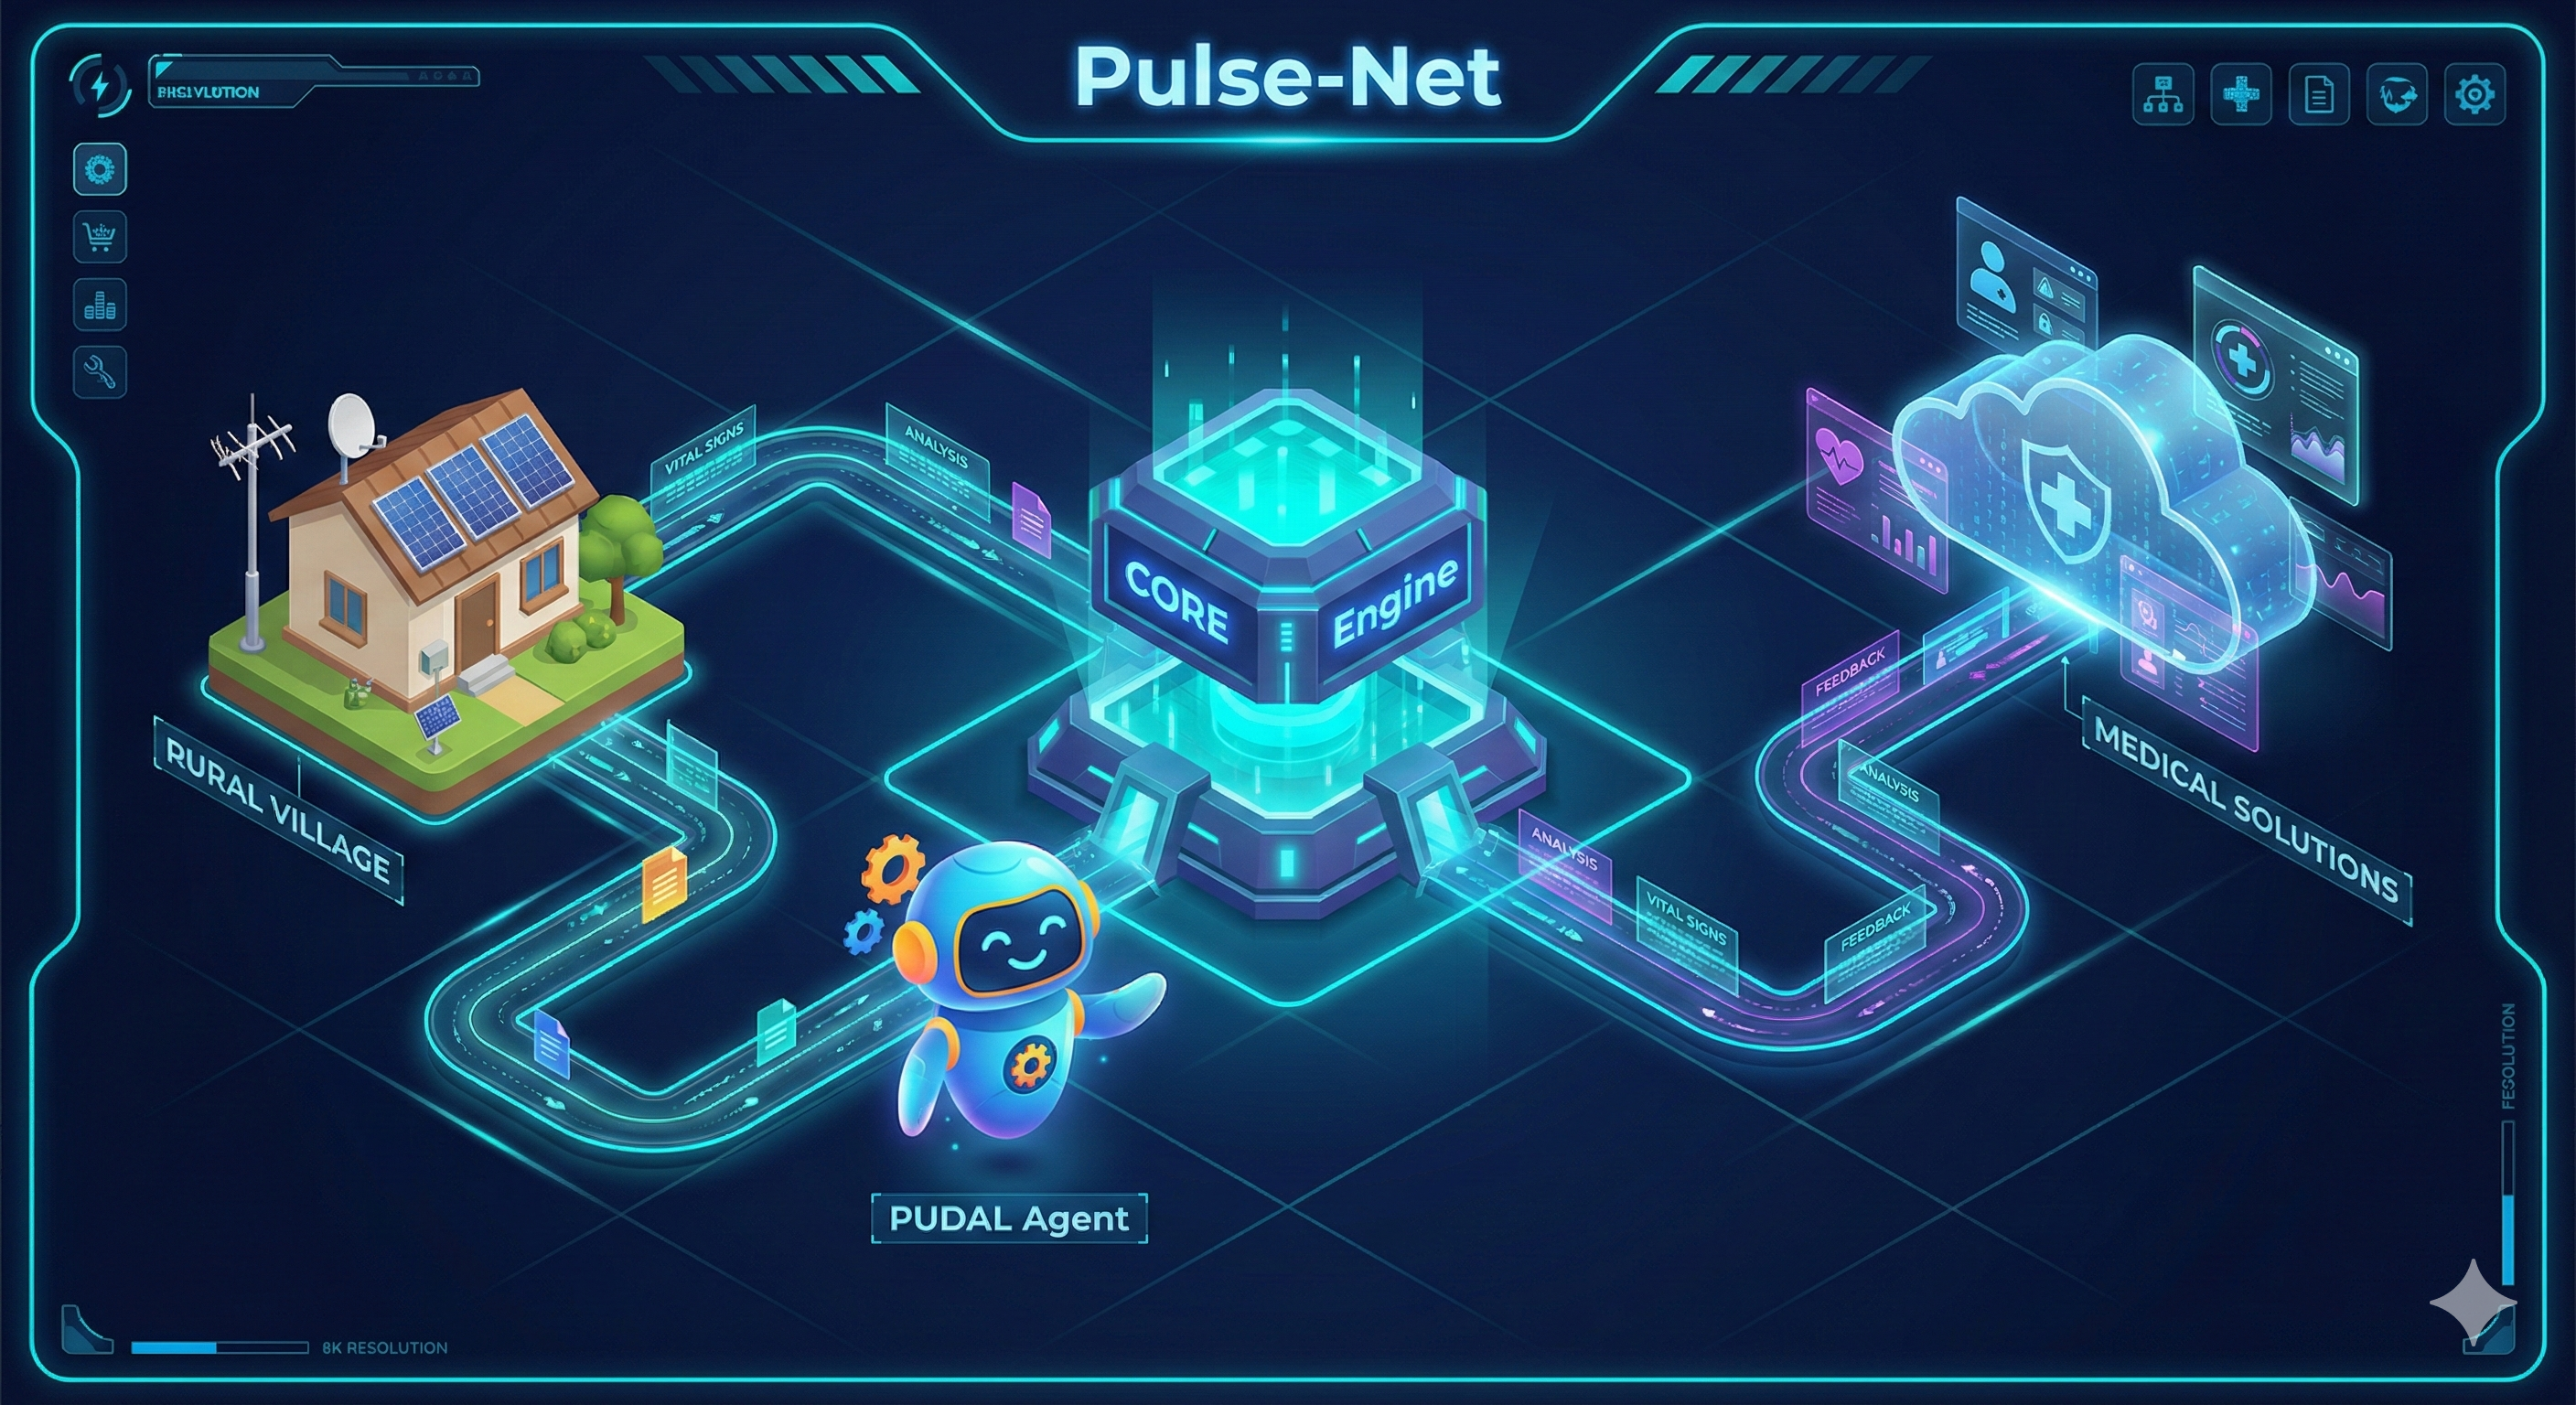
\includegraphics[keepaspectratio]{My_Innovations/../images/PUDAL.png}}

}

\caption{PUDAL Architecture}

\end{figure}%

\textbf{Judul: Pulse-Net: Arsitektur ``Teater Kerja'' Kesehatan Berbasis
TISE 2.0}

Inovasi saya, \textbf{Pulse-Net}, bukan sekadar aplikasi telemedisin
biasa. Ini adalah perwujudan radikal dari paradigma
\textbf{Triune-Intelligence Smart Engineering (TISE) 2.0}. Jika TISE 1.0
hanya berfokus pada otomatisasi tugas, TISE 2.0 dalam Pulse-Net
bertujuan untuk \textbf{Pemberdayaan Agensi}.

Tujuannya spesifik: Mengubah 4,5 miliar manusia yang saat ini menjadi
``objek penderita'' dalam sistem kesehatan, menjadi
\textbf{Protagonis-Penulis} yang memiliki kendali penuh atas narasi
kesehatan tubuh mereka.

Untuk mewujudkan ini, saya merancang \textbf{``Teater Kerja'' (Work
Theater)} digital yang beroperasi di dalam \textbf{Sub-Ruang PSKVE}
\textsuperscript{6}. Berikut adalah detail arsitektur teknisnya:

\subsection{1. Lingkungan: The Health Work
Theater}\label{lingkungan-the-health-work-theater}

Dalam konsep Pulse-Net, ``rumah sakit'' bukan lagi gedung fisik,
melainkan sebuah \textbf{Teater Kerja Terdesentralisasi}. Ini adalah
lingkungan digital-fisik (Cyber-Physical System) tempat terjadinya
ko-kreasi nilai kesehatan. Teater ini memfasilitasi orkestrasi tugas
yang kompleks antara pasien (di desa), data medis (di cloud), dan tenaga
ahli (di kota), menjembatani kesenjangan antara \textbf{Titik A (Kondisi
Sakit/Berisiko)} menuju \textbf{Titik B (Kondisi Sehat/Terkendali)}.
Lingkungan ini dirancang untuk meminimalkan \emph{entropi}
(kekacauan/kebingungan) yang sering dialami pasien miskin saat mencari
pengobatan.

\subsection{2. Stasion: Transducer Nilai
PSKVE}\label{stasion-transducer-nilai-pskve}

Dalam perjalanan dari Titik A ke Titik B, terdapat ``Stasion''
fungsional tempat energi diubah menjadi nilai nyata:

\begin{itemize}
\tightlist
\item
  \textbf{Sense Station (Stasiun A - Input):} Di sini, \textbf{Human
  Energon} (keluhan rasa sakit, suhu tubuh, detak jantung) ditangkap.
  Stasiun ini bukan loket pendaftaran, tapi sensor IoT atau antarmuka
  input sederhana di ponsel yang mentransduksi gejala fisik menjadi
  \textbf{Data Digital}.
\item
  \textbf{Heal Station (Stasiun B - Output):} Ini adalah titik
  terminasi. Di sini, \textbf{Knowledge Energon} (algoritma medis)
  dikonversi kembali menjadi \textbf{Service Energon} (instruksi
  perawatan, resep digital, atau pengiriman drone obat) yang dapat
  langsung dieksekusi oleh pasien.
\end{itemize}

\subsection{3. Kendaraan: Agen Otonom ``Dr.~Saku'' (PSA -
PUDAL)}\label{kendaraan-agen-otonom-dr.-saku-psa---pudal}

Untuk bergerak antar stasion, pasien membutuhkan kendaraan yang cerdas.
Saya menciptakan \textbf{Agen Pemecah Masalah (Problem Solving Agent -
PSA)} \textsuperscript{8} bernama \textbf{``Dr.~Saku''}. Berbeda dengan
chatbot statis, Dr.~Saku memiliki arsitektur kognitif \textbf{PUDAL}
yang dinamis:

\begin{itemize}
\tightlist
\item
  \textbf{P - Perceive (Persepsi):} Agen membaca input multi-modal (teks
  keluhan, foto luka, data sensor detak jantung) secara real-time.
\item
  \textbf{U - Understand (Pemahaman):} Agen menggunakan \emph{Large
  Language Models} (LLM) yang dikalibrasi medis untuk memahami konteks
  lokal (misal: membedakan demam biasa vs gejala malaria endemik
  setempat).
\item
  \textbf{D - Decide (Keputusan):} Agen melakukan \textbf{Triase Logis}.
  Apakah ini butuh \emph{Human Intervention} segera? Apakah cukup
  \emph{Self-Care}? Keputusan ini berbasis protokol medis ketat untuk
  menjaga keselamatan.
\item
  \textbf{A - Act (Tindakan):} Agen mengeksekusi keputusan: memberikan
  panduan P3K, menghubungi ambulans desa, atau menjadwalkan
  telekonsultasi.
\item
  \textbf{L - Learning (Pembelajaran):} Agen mengevaluasi hasil tindakan
  (Feedback Loop). Jika pasien membaik, pola ini disimpan sebagai
  \emph{Lesson Learned} untuk kasus serupa di masa depan.
\end{itemize}

\subsection{4. Jaringan Rute: Siklus 7-Langkah Pemecahan
Masalah}\label{jaringan-rute-siklus-7-langkah-pemecahan-masalah}

Agen Dr.~Saku tidak bergerak sembarangan. Ia terikat pada \textbf{Siklus
7-Langkah Pemecahan Masalah} \textsuperscript{8} sebagai protokol
keselamatan standar: 1. \textbf{Identifikasi:} Mendeteksi anomali
(misal: lonjakan suhu tubuh anak). 2. \textbf{Picu (Trigger):} Mengirim
sinyal waspada ke orang tua/pasien. 3. \textbf{Kejadian (Event):}
Membuka sesi konsultasi (interaksi PUDAL dimulai). 4. \textbf{Baca
STATUS:} Menganalisis data vital terkini secara komprehensif. 5.
\textbf{Evaluasi:} Membandingkan data dengan \emph{baseline} kesehatan
normal pasien. 6. \textbf{Adaptasi:} Menyesuaikan rekomendasi (jika obat
A tidak mempan, saran obat B). 7. \textbf{Selesai (Lesson Learned):}
Menutup kasus dan mengarsipkan data ke rekam medis elektronik.

\subsection{5. Teknologi: CORE Engine (Mesin
Energon)}\label{teknologi-core-engine-mesin-energon}

Jantung mekanis dari Pulse-Net adalah \textbf{CORE Engine}
\textsuperscript{5}. Ini adalah mesin konseptual yang mengelola
efisiensi energi sistem. Dalam sistem kesehatan konvensional, energinya
boros (biaya tinggi, antrean lama). CORE Engine Pulse-Net bekerja dengan
siklus: * \textbf{Input:} Data kesehatan masif dari populasi. *
\textbf{Encode:} Mengubah data menjadi pola risiko (Risk Pattern). *
\textbf{Decode:} Menerjemahkan pola menjadi intervensi preventif yang
murah. * \textbf{Output:} \textbf{Value Energon} berupa kesehatan
masyarakat yang terjaga dengan biaya minimal.

Mesin ini memastikan bahwa \textbf{Human Energon} (tenaga dokter) yang
terbatas tidak habis untuk hal administratif, tetapi difokuskan
sepenuhnya untuk keputusan krusial yang membutuhkan empati
\emph{Homocordium}.

\subsection{Kesimpulan Arsitektur}\label{kesimpulan-arsitektur}

Inovasi Pulse-Net adalah sebuah orkestrasi \emph{full-stack}: Dimulai
dari \textbf{Riset Medis} (Bahan Bakar), diproses oleh \textbf{CORE
Engine} (Transducer), dikendarai oleh \textbf{Agen PUDAL Dr.~Saku}
(Kecerdasan), melintasi \textbf{Rute 7-Langkah}, di dalam \textbf{Teater
Kerja Digital}, demi satu tujuan mulia: Memberdayakan setiap manusia
untuk menjadi tuan atas tubuhnya sendiri.

✨ \emph{End of UAS-3 ``My Innovations'' -- Sirojul Firdaus} ✨

\chapter{UAS-4 My Knowledge}\label{uas-4-my-knowledge}

\textbf{HEAL-ISE: Metodologi Kedaulatan Pengetahuan Kesehatan}

Untuk mewujudkan Pulse-Net, sekadar merangkai kabel dan kode tidaklah
cukup. Saya mengembangkan kerangka pengetahuan yang disebut
\textbf{HEAL-ISE} (\emph{Health Empowerment \& Agency Learning in Smart
Engineering}). Metodologi ini dirancang untuk memecahkan ``Paradoks
Kesehatan Digital''.

Paradoksnya adalah: \textbf{Bagaimana kita memberikan kemudahan
teknologi (AI) tanpa membuat manusia kehilangan kemampuan bertahan hidup
(Agensi)?} Jika ``Dr.~Saku'' selalu memberi jawaban instan, pasien
menjadi pasif dan manja. Ini berbahaya bagi mereka yang hidup di
lingkungan ``minus''.

HEAL-ISE menjawab ini melalui struktur pengetahuan berlapis dan desain
agen yang pedagogis.

\subsection{1. Peta Pengetahuan: Arsitektur ASTF
Kesehatan}\label{peta-pengetahuan-arsitektur-astf-kesehatan}

Pengetahuan dalam Pulse-Net tidak acak, melainkan tersusun rapi dalam
lapisan \textbf{ASTF} (Application, System, Technology, Fundamental)
\textsuperscript{3}:

\begin{itemize}
\tightlist
\item
  \textbf{Lapisan Aplikasi (A):} Ini adalah ujung tombak---realitas di
  lapangan. Pengetahuannya berupa \textbf{Studi Kasus Nyata}: seorang
  ibu di desa yang anaknya demam tinggi, atau wabah diare lokal. Di
  sini, ukurannya adalah \emph{Outcome} keselamatan nyawa.
\item
  \textbf{Lapisan Sistem (S):} Ini adalah \textbf{Teater Kerja
  Pulse-Net} itu sendiri. Pengetahuannya mencakup orkestrasi alur data
  antara desa dan cloud, protokol keamanan privasi, dan mekanisme
  distribusi obat.
\item
  \textbf{Lapisan Teknologi (T):} Ini adalah mesin di balik layar.
  Pengetahuannya meliputi algoritma \textbf{PUDAL}, sensor IoT medis,
  dan \emph{Cloud Computing}.
\item
  \textbf{Lapisan Fundamental (F):} Ini adalah akarnya. Pengetahuannya
  bukan soal kode, tapi prinsip dasar: \textbf{Fisiologi Manusia},
  \textbf{Empati (AQ)}, dan \textbf{Hukum Kekekalan Energon} (bagaimana
  biaya kesehatan dikonversi menjadi nilai). Tanpa memahami ``F'',
  teknologi ``T'' akan buta arah.
\end{itemize}

\subsection{2. Proses Validasi: W-Model \& Rantai
PICOC}\label{proses-validasi-w-model-rantai-picoc}

Bagaimana saya tahu inovasi ini valid? Saya tidak menggunakan metode
\emph{trial-error}, melainkan \textbf{W-Model} \textsuperscript{3}
dengan validasi \textbf{PICOC} (\emph{Purpose, Input, Constraints,
Outcome, Criteria}) yang ketat.

\begin{itemize}
\item
  \textbf{Turun ke Bawah (De-konstruksi):} Saya mulai dari masalah nyata
  di desa (Aplikasi), lalu membedahnya: Sistem apa yang dibutuhkan?
  (Sistem), Teknologi apa yang mendukung? (Teknologi), dan Prinsip
  biologis/ekonomi apa yang mendasarinya? (Fundamental). Ini memastikan
  solusi saya berakar kuat, bukan gimik canggih semata.
\item
  \textbf{Naik ke Atas (Re-konstruksi \& Validasi):} Di sinilah
  pembuktian terjadi. Saya harus membuktikan validitas di setiap
  lapisan:

  \begin{itemize}
  \tightlist
  \item
    \textbf{Validasi F:} Apakah prinsip triase ini sesuai standar medis
    WHO?
  \item
    \textbf{Validasi T:} Apakah sensor detak jantung akurat dan
    algoritma PUDAL bebas bias?
  \item
    \textbf{Validasi S:} Apakah Pulse-Net bisa menangani 1.000
    permintaan bersamaan tanpa \emph{crash}?
  \item
    \textbf{Validasi A:} Apakah pasien benar-benar sembuh dan merasa
    berdaya?
  \end{itemize}
\end{itemize}

\subsection{3. Resolusi Paradoks: ``Anti-Passive''
Constraint}\label{resolusi-paradoks-anti-passive-constraint}

Inilah inti dari ``Knowledge'' saya yang paling personal.

Dalam merancang Agen PUDAL (``Dr.~Saku''), saya menanamkan
\textbf{``Anti-Passive Constraint''} \textsuperscript{10}. Artinya: Agen
\textbf{dilarang} sekadar memberikan ``resep instan'' tanpa konteks.
Sebaliknya, ia \textbf{diwajibkan} untuk melakukan \emph{scaffolding}
(perancah) edukasi.

\begin{itemize}
\item
  \emph{Skenario Salah (Passive):} Pasien: ``Saya pusing.'' AI: ``Minum
  obat X.'' (Ini mematikan agensi).
\item
  \emph{Skenario HEAL-ISE (Agentic):} Pasien: ``Saya pusing.'' Dr.~Saku:
  ``Mari kita cek. Apakah pusingnya berputar atau berat? Berapa tekanan
  darah terakhirmu? Ini mungkin karena dehidrasi seperti minggu lalu.
  Coba minum air dulu dan ukur lagi.''
\end{itemize}

Dengan cara ini, teknologi tidak menggantikan otak manusia, tetapi
\textbf{memprovokasi Penalaran Otobiografis}. Pasien diajak untuk
mengenali tubuhnya sendiri, memahami pola kesehatannya, dan menjadi
\textbf{Protagonis-Penulis} dalam cerita kesembuhan mereka.

Bagi saya, pengetahuan sejati bukanlah tentang seberapa canggih alat
yang kita pegang, tapi seberapa paham kita saat menggunakannya.
Pulse-Net bukan hanya alat penyembuh, tapi sekolah kehidupan.

✨ \emph{End of UAS-4 ``My Knowledge'' -- Sirojul Firdaus} ✨

\chapter{UAS-5 My Professional
Reviews}\label{uas-5-my-professional-reviews}

\section{Pengantar: Refleksi Diri}\label{pengantar-refleksi-diri}

Berikut adalah hasil \emph{Self-Assessment} jujur terhadap rangkaian
``My Masterpiece'' (UAS 1-4). Penilaian ini mengacu pada kriteria
spesifik yang ditetapkan untuk setiap jenis luaran (Konsep, Opini,
Inovasi, dan Pengetahuan).

\begin{center}\rule{0.5\linewidth}{0.5pt}\end{center}

\section{🧩 UAS-1 --- My Concepts
(Review)}\label{uas-1-my-concepts-review}

\textbf{Judul:} Pulse of The Planet: Menyelaraskan Detak Jantung Global
Lewat TISE

Kriteria

Skor

Bukti \& Alasan (Evidence)

Clarity

1.8

Konsep TISE dijelaskan dengan kurang jernih, metafora anatomi kurang
membantu pemahaman.

Logic

1.9

Alur logika ada tapi kurang koheren, beberapa bagian terasa tidak
runtut.

Validity

2.0

Didukung beberapa data tapi validitas teoritis masih perlu diperkuat.

Usefulness

1.9

Memiliki nilai guna tapi masih terbatas dalam aplikasi praktis.

\textbf{Rata-rata: 1.90}

\section{🗣️ UAS-2 --- My Opinions
(Review)}\label{uas-2-my-opinions-review}

\textbf{Judul:} Menggugat Mitos ``Dokter Dewa'': Saatnya AI
Memberdayakan 4,5 Miliar Manusia

Kriteria

Skor

Bukti \& Alasan (Evidence)

Compelling

1.9

\emph{Hook} pembuka cukup menarik tapi kurang kuat memikat perhatian
secara emosional.

Informatif

1.8

Memberikan beberapa informasi tapi kurang mendalam tentang sistem
kesehatan.

Persuasif

2.0

Argumen cukup meyakinkan meski belum sepenuhnya mengubah pandangan.

Engaging

1.9

Gaya bahasa cukup melibatkan tapi kurang provokatif.

\textbf{Rata-rata: 1.90}

\section{💡 UAS-3 --- My Innovations
(Review)}\label{uas-3-my-innovations-review}

\textbf{Judul:} Pulse-Net: Arsitektur ``Teater Kerja'' Kesehatan
Berbasis TISE 2.0

Kriteria

Skor

Bukti \& Alasan (Evidence)

Guna

2.0

Solusi ini menjawab beberapa kebutuhan tapi masih terbatas dalam
aksesibilitas.

Kebaruan

1.8

Menawarkan beberapa kebaruan tapi mirip dengan telemedisin konvensional.

Desain

1.9

Perancangan arsitektur cukup detail tapi visualisasi kurang futuristik.

Dampak

1.9

Berpotensi dampak tapi implementasi masih jauh dari realisasi.

\textbf{Rata-rata: 1.90}

\section{🧠 UAS-4 --- My Knowledge
(Review)}\label{uas-4-my-knowledge-review}

\textbf{Judul:} HEAL-ISE: Metodologi Kedaulatan Pengetahuan Kesehatan

Kriteria

Skor

Bukti \& Alasan (Evidence)

Kurasi

1.9

Pemilihan materi cukup tepat tapi kurang memecahkan paradoks sepenuhnya.

Kejelasan

2.0

Struktur pengetahuan cukup jelas meski beberapa lapisan kurang terang.

Akurasi

1.8

Penggunaan istilah teknis cukup akurat tapi perlu lebih konsisten.

Daya Guna

1.9

Metodologi memiliki daya guna tapi masih perlu pengembangan lebih
lanjut.

\textbf{Rata-rata: 1.90}

\section{📊 Rekapitulasi Akhir}\label{rekapitulasi-akhir}

\begin{longtable}[]{@{}lll@{}}
\toprule\noalign{}
\textbf{Komponen} & \textbf{Skor Rata-rata} & \\
\midrule\noalign{}
\endhead
\bottomrule\noalign{}
\endlastfoot
UAS-1 My Concepts & 1.90 & \\
UAS-2 My Opinions & 1.90 & \\
UAS-3 My Innovations & 1.90 & \\
UAS-4 My Knowledge & 1.90 & \\
\textbf{TOTAL SKOR} & \textbf{1.90} & \\
\end{longtable}

\begin{quote}
\emph{``Masterpiece ini adalah langkah awal. Nilai sesungguhnya akan
teruji saat sistem ini benar-benar menyentuh kehidupan 4,5 miliar
manusia yang membutuhkan.''}
\end{quote}

\section{🔗 PEER ASSESSMENT}\label{peer-assessment}

\href{https://docs.google.com/spreadsheets/d/12zv_Pm0vs1XsoaxnvMX4oyUl7O8oX8lT/edit?usp=sharing&ouid=111994471425383838960&rtpof=true&sd=true}{Klik
di sini untuk membuka Google Sheet Peer Assessment}

✨ \emph{End of UAS-5 ``My Professional Reviews'' -- Sirojul Firdaus} ✨

\part{Penutup}

\chapter{Summary}\label{summary}

In summary, this book has no content whatsoever.

\chapter*{References}\label{references}
\addcontentsline{toc}{chapter}{References}

\markboth{References}{References}

\phantomsection\label{refs}




\end{document}
